\documentclass[a4paper,12pt]{scrreprt}
\usepackage[utf8]{inputenc}
\usepackage[ngerman, english]{babel}
\selectlanguage{ngerman}
\usepackage[T1]{fontenc}
\usepackage{lmodern}
\usepackage[babel, german=quotes]{csquotes}
%\usepackage{hyperref}
\usepackage[style=authoryear, natbib, backend=biber]{biblatex}
\usepackage[top=3cm,bottom=3cm,left=2cm,right=2cm]{geometry}
\usepackage{listings}
\usepackage{hyperref}
\usepackage{graphicx, fancyhdr, array, wrapfig, colortbl, algorithm, algpseudocode, subcaption, setspace}
\usepackage[usenames,dvipsnames]{xcolor}
\usepackage{pgfgantt}
\usepackage{pdflscape}
\usepackage{amsfonts}
\usepackage{tikz}
\usetikzlibrary{arrows,shapes,positioning,shadows,trees}
\floatname{algorithm}{Algorithmus}
\renewcommand{\listalgorithmname}{Algorithmenverzeichnis}
\renewcommand{\algorithmicend}{\textbf{Ende}}
\renewcommand{\algorithmicif}{\textbf{Falls}}
\renewcommand{\algorithmicthen}{\textbf{dann}}
\renewcommand{\algorithmicelse}{\textbf{Sonst}}
\renewcommand{\algorithmicdo}{\textbf{}}
\renewcommand{\algorithmicwhile}{\textbf{Solange}}
\renewcommand{\algorithmicreturn}{\textbf{Returniere}}
\renewcommand{\algorithmicrequire}{\textbf{Eingabe}}
\renewcommand{\algorithmicensure}{\textbf{Ausgabe}}
\renewcommand{\algorithmicforall}{\textbf{Für alle}}
\renewcommand{\algorithmicfor}{\textbf{Für}}

\newcommand{\ap}[1]{\ensuremath{\mathfrak{#1}}}

\newcolumntype{L}[1]{>{\raggedright\let\newline\\\arraybackslash\hspace{0pt}}m{#1}}
\newcolumntype{C}[1]{>{\centering\let\newline\\\arraybackslash\hspace{0pt}}m{#1}}
\newcolumntype{R}[1]{>{\raggedleft\let\newline\\\arraybackslash\hspace{0pt}}m{#1}}


\lstdefinestyle{customc}{
  belowcaptionskip=1\baselineskip,
  breaklines=true,
  xleftmargin=\parindent,
  numbers=left,
  language=C++,
  showstringspaces=false,
  basicstyle=\footnotesize\ttfamily,
  keywordstyle=\bfseries\color{OliveGreen},
  commentstyle=\itshape\color{purple},
  identifierstyle=\color{blue},
  stringstyle=\color{orange},
  frame=tb,
  stepnumber=1,
  tabsize=4,
  postbreak=\raisebox{0ex}[0ex][0ex]{\ensuremath{\hookrightarrow\ \ }},
  numberstyle=\scriptsize,
  breakatwhitespace=true,
  breaklines=true,
}
\lstset{style=customc}
%\renewcommand\familydefault{\sfdefault}
\linespread{1.5}
\setlength{\parindent}{4mm}
\setlength{\parskip}{2mm}
\pagestyle{fancy}
\fancyhf{}
\clubpenalty = 300
\widowpenalty = 300
\displaywidowpenalty = 300
\fancyfoot{}
\fancyhead{}
\renewcommand{\footrulewidth}{0.4pt}
\rfoot{{\footnotesize \textnormal{\thepage}}}
\lhead{{\footnotesize \textnormal{\thesection}}}
\chead{{\footnotesize \textnormal{Variable Neighborhood Search für das Partition Graph Coloring Problem}}}
\cfoot{{\footnotesize \textnormal{Lorenz Leutgeb, Moritz Wanzenböck}}}
\lfoot{{\footnotesize \textnormal{\the\year}}}
\addbibresource{../pcp.bib}
\let\origappendix\appendix
\let\origthesection\thesection
\renewcommand\appendix{\clearpage\pagenumbering{roman}\origappendix}
\renewcommand{\lstlistlistingname}{Codeverzeichnis}
% Graphiken in ../img/
% \cite{Lu2010, Palladino2011, Noronha2006, Li2000, Frota2010, Demange, pcp-instance-page}

\title{Variable Neighborhood Search für das Partition Graph Coloring Problem}
\author{Lorenz Leutgeb, Moritz Wanzenböck}

\begin{document}
\begin{titlepage}
\begin{center}

\includegraphics[height=2cm]{../img/htl.png}

\vspace{10mm}

{\Large D}\ {\large I\ P\ L\ O\ M\ A\ R\ B\ E\ I\ T}

\vspace{25mm}

{\Huge\bfseries\sffamily Variable Neighborhood Search}\\[3mm]
{\Huge\bfseries\sffamily für das}\\[3mm]
{\Huge\bfseries\sffamily Partition Graph Coloring Problem}

\vspace{15mm}

ausgeführt unter der Leitung von

\vspace{5mm}

{\large\bfseries Mag.~rer.~soc.~oec.\ Dipl.-Ing.\ Dr.~techn.\ Martin Gruber}

\vspace{5mm}

eingereicht an der

\vspace{5mm}

{\large Höheren Technischen Bundeslehr- und Versuchsanstalt Wien Ottakring}

{\large Abteilung für Informationstechnologie und Elektronik}

\vspace{5mm}

von

\vspace{5mm}
\begin{tabular}{>{\raggedright\arraybackslash}p{.3\textwidth}c>{\raggedleft\arraybackslash}p{.3\textwidth}}
{\large\bfseries Lorenz Leutgeb} & und & {\large\bfseries Moritz Wanzenböck} \\
\end{tabular}
\end{center}
\vspace*{\fill}

Wien, am 8.~Mai 2013
\end{titlepage}

\newgeometry{margin = 0cm}
\begin{center}
\vspace*{\fill}

\includegraphics[height=0.95\textheight]{../img/antrag.jpg}
\vspace*{\fill}
\end{center}
\thispagestyle{empty}
\restoregeometry

\addcontentsline{toc}{chapter}{Eigenständigkeitserklräung}
\vspace*{\fill}
\section*{Eigenständigkeitserklärung}

Hiermit erklären wir, Lorenz Leutgeb und Moritz Wanzenböck, an Eides statt, dass wir die vorliegende Diplomarbeit selbstständig und nur mit den angegebenen Hilfsmitteln verfasst haben.

Wir versichern ausdrücklich, dass sämtliche in der Arbeit verwendeten fremden Quellen, auch aus dem Internet, als solche kenntlich gemacht wurden. Insbesondere bestätigen wir, dass ausnahmslos sowohl bei wörtlich übernommenen Aussagen bzw.\ unverändert übernommenen Tabellen, Grafiken u.~Ä.\ (Zitaten) als auch bei in eigenen Worten wiedergegebenen Aussagen bzw.\ von uns abgewandelten Tabellen, Grafiken u.~Ä.\ anderer Autorinnen und Autoren (indirektes Zitieren) die entsprechende Quelle angegeben wurde.

Uns ist bewusst, dass Verstöße gegen die Grundsätze der Selbstständigkeit als Täuschung betrachtet und entsprechend der Gesetzgebung geahndet werden.

Die vorliegende Arbeit wurde in gleicher oder ähnlicher Form bisher bei keiner anderen Institution eingereicht.

\vspace{3cm}

\begin{center}
\begin{tabular}{ccc}
    \rule{0.4\textwidth}{0.5pt} & \hspace{5mm} & \rule{0.4\textwidth}{0.5pt} \\
    Lorenz Leutgeb & & Moritz Wanzenböck
\end{tabular}
\end{center}
\vspace*{\fill}
\addcontentsline{toc}{chapter}{Eigenständigkeitserklärung}

\addcontentsline{toc}{chapter}{Abstract}
\vspace*{\fill}
\section*{Abstract}
Lipsum dolor sit amet in conspexitur ad domus entratum de regio. Filius clarus maloribus adveniens ex Clarisses.
\vspace*{\fill}

\tableofcontents
\newpage
\chapter{Problemstellung}
In der heutigen Zeit, in der das weltweite Kommunikationsbedürfnis in ungeahnte Höhen steigt und, bis auf Weiteres, kein Ende des Anstiegs in Sicht ist, werden Computer-Netzwerke, besonders jene, welche ganze Kontinente umspannen, immer stärker beansprucht. Dieser Anstieg ist vor allem auf das gesteigerte und sich grundlegend ändernde Konsumverhalten der Menschen in der heutigen Zeit zurückzuführen. Immer mehr Informationen in Netzwerken werden nicht in Form von Texten sondern, aufwendig aufbereitet, als Bild und Ton zum Endkunden übertragen. Dieses Bild- und Tonmaterial erzeugt natürlich eine höhere Auslastung von Datenleitungen, was, im Zusammenspiel mit der gestiegenen Anzahl an Informationsbedürfnissen insgesamt, zu einer Verknappung der Ressourcen in Computer-Netzen führt.

Um diesen neuen Gegebenheiten gerecht zu werden gibt es zwei Möglichkeiten: entweder ein Ausbau und Neubau von Netzen, oder eine bessere Ausnutzung von bestehenden Netzen. Ausbau und Neubau bringen allerdings neue Probleme mit sich. Erstens ist Netzwerkinfrastruktur teuer, besonders wenn sie über mehrere Jahrzehnte hinweg halten und ihren Dienst verrichten soll ohne eine ständige Wartung mit sich zu ziehen. Zweitens ist es manchmal aus verschiedenen Gründen gar nicht möglich, ein Netz weiter auszubauen. Sollte sich eine bestehende Infrastruktur bereits in ihrer letzten Ausbaustufe befinden, ist es überhaupt notwendig ein gänzlich neues Netz aufzubauen, was wiederum mit noch höheren Kosten verbunden ist. Zu guter Letzt sorgt der Betrieb von zusätzlicher Infrastruktur auch für zusätzlichen Strombedarf, was sich nicht nur negativ auf die Kosten auswirkt, sondern durchaus auch eine Belastung für die Umwelt darstellt.

Die zweite Möglichkeit, die bessere Ausnutzung von bestehenden Netzen, kann zwar die letzt\-endliche Notwendigkeit von neuen Netzen nicht verhindern, den Zeitpunkt des Eintretens dieser letzten Option aber hinauszögern. Durch eine optimierte Nutzung können bereits vorhandene Netze über einen längeren Zeitraum genutzt werden ohne einen Engpass zu bilden. Wie diese Optimierungen im konkreten Fall aussehen hängt unter anderem von der Größe und der Art des Netzes, aber auch von der Art des Kommunikationsbedürfnisses ab. In dieser Arbeit konzentrieren wir uns auf rein optische Netze mit einer ganz genau definierten Art von Kommunikationsbedürfnissen.

In rein optischen Netzen, also Netzwerken, in denen Information als Lichtimpulse rein über optische Leiter wie Glasfaser übertragen wird und das Signal auf der ganzen Strecke zu keinem Zeitpunkt in ein elektrisches Signal zurück gewandelt wird, kann \textit{Wavelength Division Multiplexing} (WDM) zur parallelen Übertragung mehrerer Datenströme über ein und dieselbe Leitung betrieben werden. Die Idee hinter WDM ist es, für zwei verschiedene Datenströme unterschiedliche Farben des Lichts zu verwenden. Der englische Name Wavelength Division (deutsch: Wellenlängen Unterteilung) kommt von der Tatsache, dass verschiedene Farben des Lichts verschiedene, eindeutige Wellenlängen haben. Da sich die unterschiedliche Farben des Lichts bei entsprechendem Wellenlängenabstand nicht gegenseitig beeinflussen, können viele Farben gleichzeitig durch ein und denselben Lichtwellenleiter geschickt werden und am anderen Ende des Leiters wieder problemlos auseinander gehalten werden. Dies funktioniert sogar so gut, dass Lichtwellen, welche sich nur um wenige Nanometer an Wellenlänge unterscheiden, immer noch eindeutig zuordenbar sind.

Des Weiteren wird oft angestrebt, einem einzelnen Datenstrom auf seinem gesamten Weg durch das Netzwerk ein und dieselbe Farbe zu geben. Dies bietet Vorteil vor allem im Bereich der Einfachheit der Implementierung, da optische Switches innerhalb des Netzwerkes keine Umwandlung von einer Farbe in eine andere vornehmen müssen. Hinzu kommt ein geringerer Stromverbrauch im Netzwerk, da ein Umwandlung von einer Wellenlänge in eine andere auch ein gewisses Maß an zusätzlicher Energie benötigen würde.

Zu guter Letzt ist noch die spezielle Art des Kommunikationsbedürnisses zu beachten. Anders als zum Beispiel im Internet, wo die Kommunikation für einen Netzbetreiber unberechen- und vor allem unverhersehbar abläuft, gehen wir hier von einem Fall aus, in dem ein großter Teil der Kommunikationswünsche bereits von vornherein bekannt sind. Vorstellbar wäre solch ein Fall zum Beispiel bei einer gemieteten Standleitung eines Unternehmens zu dessen Zweigstelle am anderen Ende des Landes. Auch die Kommunikationsbedürfnisse zwischen Internetprovidern (z.\ B. Durchleitung von Daten) können im großen Maßstab als ein über einige Wochen oder Monate hinweg relativ konstantes Datenaufkommen betrachtet werden. Obwohl dies nun nach einer starken Einschränkung des Einsatzgebietes aussieht ist der Nutzen dennoch nicht zu unterschätzen. Wenn zum Beispiel der Aufwand für den Betrieb solcher Standleitungen minimiert werden kann, bleiben mehr Ressourcen des Netzwerkes frei für die Erfüllung der vorhin erwähnten unvorhersehbaren Kommunikationsbedürfnisse.

\section{Partition Graph Coloring Problem}
Mit Hilfe des \textit{Partition Graph Coloring Problems} (PCP) wird versucht, diesen sehr spezifischen Anwendungsfall mathematisch zu beschreiben. Um das Problem zu lösen wird ein Graph aufgebaut, mit dessen Hilfe dann eine möglichst gute, wenn nicht sogar optimale Lösung für das Problem berechnet werden kann. Ein Graph ist ein mathematisches Konstrukt, das aus Knoten besteht, die durch Kanten verbunden werden. Ein Knoten A kann mit Knoten B durch so eine Kante verbunden werden, Knoten A muss aber zum Beispiel keine Verbindung mit Knoten C besitzen. Wie schon von \citet*{Li2000} gezeigt wurde, handelt es sich bei dem PCP um ein NP-hartes Problem, das heißt es kann nicht in polynomieller Laufzeit auf einem Computer wie man ihn heute kennt eine Lösung gefunden werden, welche mit 100\%-iger Sicherheit die optimale Lösung für das konkrete Problem darstellt. Polynomielle Laufzeit wird im Normalfall als Grenze zwischen Problemen angesehen, welche in vertretbarer Laufzeit noch zu berechnen sind und Problemen, für die der Lösungsaufwand in keinem Verhältnis zum Ergebnis steht, namentlich, deren Laufzeit ein exponentielles Verhalten an den Tag legt.

\begin{figure}
	\centering
	\begin{subfigure}{\textwidth}
		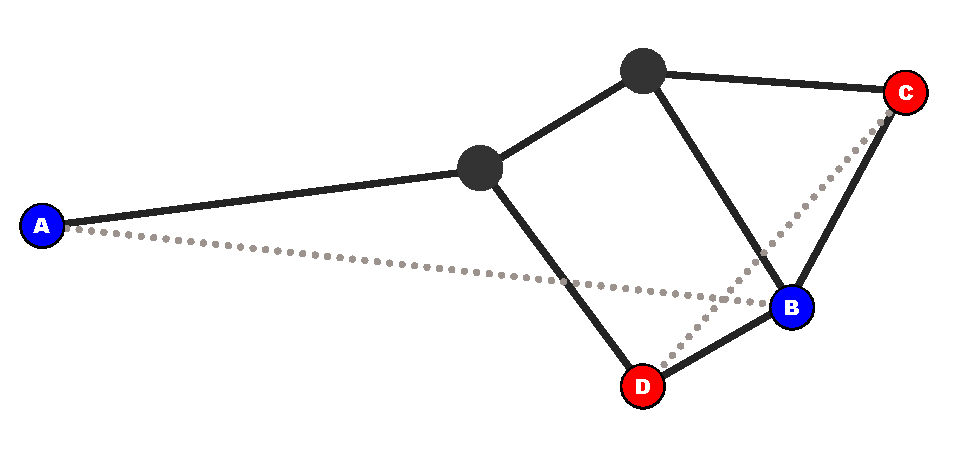
\includegraphics{img/bsp1}
		\caption{Repräsentatives Beispiel für ein rein optisches Netzwerk innerhalb Österreichs. Es gibt zwei Kommunikationswünsche und zwar zwischen A und B sowie zwischen C und D.}
		\label{fig:example:a}
	\end{subfigure}
	\begin{subfigure}{\textwidth}
		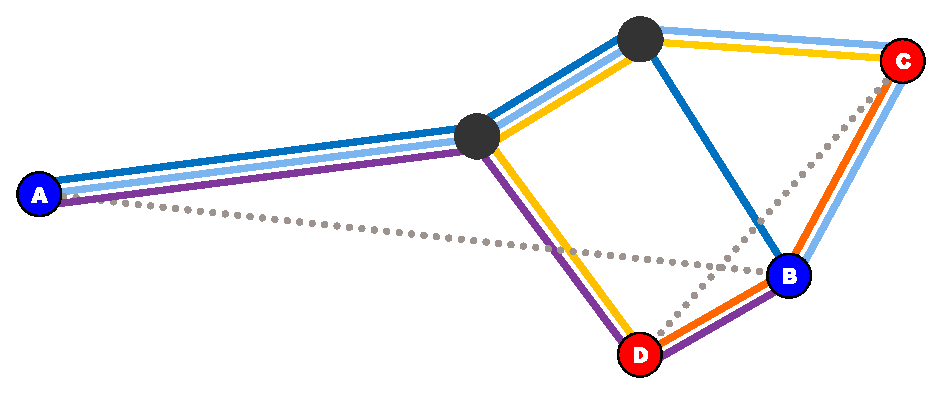
\includegraphics{img/bsp2}
		\caption{Beispiel für verschiedene Routen zwischen insgesamt vier Kommunikationspartnern. Verschiedene Möglichkeiten der Wegfindung zwischen A und B werden in Hell- und Dunkelblau sowie Violett dargestellt. Die alternativen Routen zwischen C und D sind gelb und orange eingefärbt.}
		\label{fig:example:b}
	\end{subfigure}
	\caption{Ein Beispiel für eine Probleminstanz des Partition Graph Coloring Problems}
	\label{fix:example}
\end{figure}

\begin{figure}
	\centering
	\begin{subfigure}[t]{0.3\textwidth}
		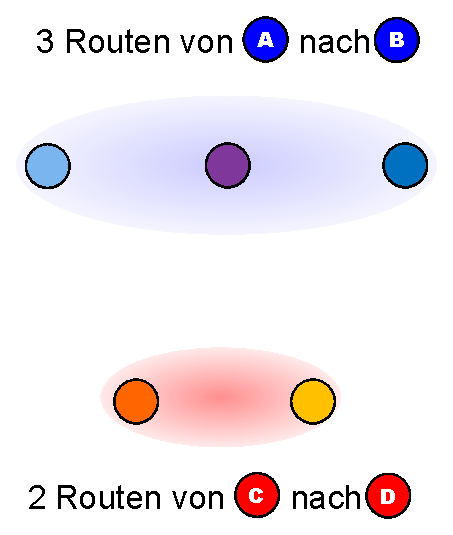
\includegraphics[width=\textwidth]{img/bsp3}
		\caption{Der aus Abbildung~\ref{fig:example:b} generierte Konfliktgraph. Jede Route wird als Knoten repräsentiert. Die verwendete Farbe stimmt mit den für die Routen verwendeten Farben überein. Die Partitionierung wird durch das Oval im Hintergrund der Knoten angedeutet.}
		\label{fig:example:c}
	\end{subfigure}
	\begin{subfigure}[t]{0.3\textwidth}
		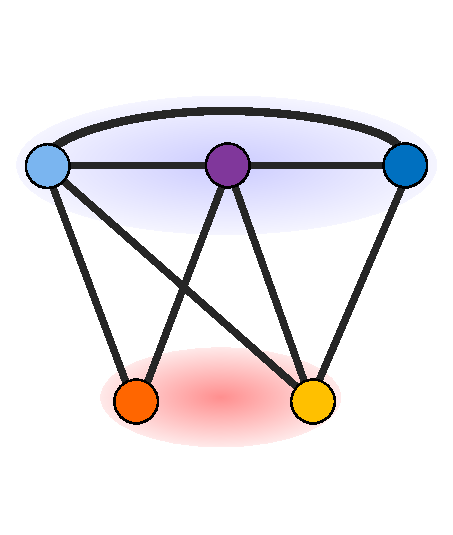
\includegraphics[width=\textwidth]{img/bsp4}
		\caption{Der Konfliktgraph wird um die Beziehungen der Knoten untereinander erweitert. Jede Route, welche eine Teilstrecke mit einer anderen Route gemeinsam hat, wird mit dieser Route verbunden. Die Kanten zwischen den Knoten stellen diese Beziehung dar.}
		\label{fig:example:d}
	\end{subfigure}
	\begin{subfigure}[t]{0.3\textwidth}
		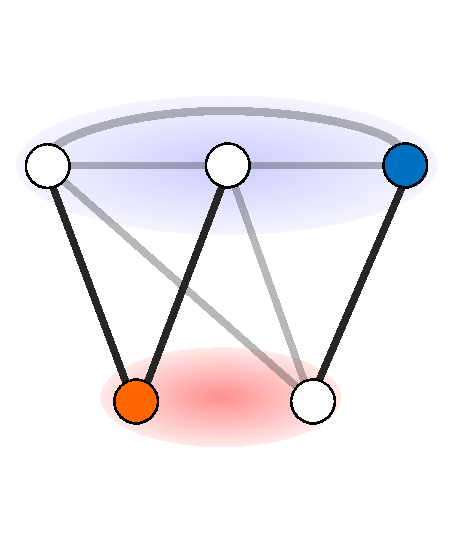
\includegraphics[width=\textwidth]{img/bsp5}
		\caption{Eine mögliche Lösung des PCP\@. Von jeder Partition muss nur ein Knoten ausgewählt werden, alle anderen werden ausgeblendet. Die Auswahl für die Strecke zwischen A und B hat kein gemeinsames Teilstück mit der für die Strecke C-D getroffenen Auswahl. Daher kann ein und dieselbe Wellenlänge für beide Übertragungen verwendet werden.}
		\label{fig:example:e}
	\end{subfigure}
	
	\caption{Aufbau und Lösung eines Problem-Graphen des Partition Graph Coloring Problems}
\end{figure}

Um das Problem besser lösen zu können, wird ein einheitliches Ziel und eine einheitliche Eingabe benötigt. Dazu wird die Problemstellung nun in einem ersten Schritt auf folgende Punkte fixiert:
\begin{itemize}
	\item Ein Netzwerk mit seinen möglichen Kommunikationsverbindungen zwischen den einzelnen Netzwerkknoten ist gegeben.
	\item Alle Kommunikationsbedürfnisse, welche aus einem Start- und einem Endpunkt bestehen, sind bekannt.
	\item Für jedes Kommunikationsbedürfnis gibt es einen oder mehrere Wege, sprich Routen, zwischen Start- und Endpunkt durch das Netzwerk.
	\item Sollte eine Route einen Teil des Weges auf der selben Strecke zurücklegen wie eine andere Route, müssen sie unterschiedliche Farben verwenden um sich nicht gegenseitig zu stören.
	\item Jede Route verwendet genau eine Farbe und zwar für die gesamte Strecke.
	\item Die Lösung besteht aus genau einer Route für jedes Kommunikationspaar und genau einer dazugehörigen Farbe.
\end{itemize}

Aus diesen Bedingungen kann ein Graph abgeleitet werden, der genau jene Bedürfnisse erfüllt, um ein einfaches Lösen des Problems zu ermöglichen. Der Konfliktgraph, auf dem dann die Lösung berechnet wird, besteht aus Partitionen, welche eine Menge von zusammengehörigen Knoten darstellt und Kanten, welche die einzelnen Knoten verbinden. Ein Kommunikationsbedürfnis zwischen zwei Partnern wird als eine Menge von Knoten gesehen. Die Knoten repräsentieren dabei je eine Route zwischen den beiden Partnern. Steht also nur eine Route zwischen zwei Kommunikationsendpunkten zur Auswahl, gibt es nur einen Knoten in dieser Menge. Diese Menge an Knoten wird Partition genannt und ist damit namensgebend für das PCP\@. Dieser Schritt wird in Abbildung~\ref{fig:example:c} veranschaulicht.

Die Kanten bilden nun die Beziehungen zwischen verschiedenen Routen ab. Teilen sich zwei Routen das selbe Teilstück im optischen Netzwerk, werden sie mit einer Kante verbunden. Zu beachten ist, dass dies nicht nur für Knoten in der selben Partition gilt sondern auch für Knoten aus unterschiedlichen Partitionen. Verwendet also Route $X$ der Kommunikation $(AB)$ ein Stück der Strecke, das auch von der Route $Y$ der Kommunikation $(CD)$ verwendet wird, werden diese beiden Routen, welche ja jeweils als Knoten repräsentiert werden, im Konfliktgraphen mit Hilfe einer Kante verbunden. Außerdem ist noch zu beachten, dass für jedes in dieser Art verbundene Routenpaar nur eine Kante verwendet wird. Teilen sich Routen $X$ und $Y$ mehr als ein Teilstück, so werden sie trotzdem nur einmal per Kante verbunden. Die Vervollständigung des Konfliktgraphen wird in Abbildung~\ref{fig:example:d} dargestellt.

Nachdem der Konfliktgraph generiert wurde, kann eine Lösung für das PCP berechnet werden. Für das durch die Partition symbolisierte Kommunikationsbedürfnis muss genau eine Route ausgewählt werden und diese Knoten müssen dann so eingefärbt werden, dass sich keine zwei mit einer Kante verbunden Knoten die gleiche Farbe teilen. Der letztere Teil, also das Einfärben von Knoten in Abhängigkeit der Farben der Nachbarknoten, ist als klassisches \textit{Graph Coloring} (GC) bekannt. Es kommt zum Beispiel bei der Einfärbung von politischen Landkarten zum Einsatz, wo benachbarte Länder nicht die selbe Farbe haben dürfen. Was das PCP vom klassichen GC unterscheidet, ist die zusätzliche Aufgabe, nur einen Knoten aus einer Partition als Repräsentanten auszuwählen und die anderen quasi auszublenden. Ein Beispiel einer solchen Lösung des Problems ist in Abbildung~\ref{fig:example:e} zu finden.

Die Schwierigkeit des Problems liegt in dem Zusammenspiel von verschiedenen Möglichkeiten, ein und den selben Graphen einzufärben und andererseits mit einer anderen Auswahl an Knoten gleich den gesamten Lösungsgraphen zu verändern. Das Kriterium für die Güte einer Lösung ist die Anzahl der verwendeten Farben. Im Originalproblem entspricht das der Anzahl an Wellenlängen, die für die vorab bekannte Kommunikation im Netzwerk benötigt werden. Um sich nur auf diese Anzahl konzentrieren zu können, wird angenommen, dass jede Route zwischen zwei Kommunikationspartnern gleich gut ist. Eventuelle Umwege (Routen länger als die kürzeste mögliche) werden also im PCP ignoriert. 

Außerdem geht man bei der Lösung des PCP von einem homogenen Netzwerk aus, in dem jede Leitung jede Wellenlänge unterstützt. In der Realität kann es durchaus vorkommen, dass ein Lichtwellenleiter, welcher aus einem chemisch minimal anders zusammengesetzten Stoff besteht als seine Gegenstücke in anderen Teilen des Netzwerkes, für bestimmte Wellenlängen ungünstige Eigenschaften hat. Dieser Aspekt wird beim Lösen des PCP nicht beachtet, jede Strecke beziehungsweise jede Route unterstützt alle Wellenlängen. Außerdem wird angenommen, dass jeder Leiter eine unbegrenzte Anzahl an Wellenlängen unterstützt. Reale Leiter können nur eine begrenzte Anzahl an Wellenlängen unterstützen, bis ihr Spektrum ausgeschöpft ist.

\subsection{Formale Definition}

Gegeben sei ein ungerichteter Graph $G = (V,\ E)$, wobei $V$ die Menge der Knoten des Graphen $G$ und $E$ die Men\-ge der Kan\-ten, die $V$ in $G$ verbinden, darstellen. Außerdem seien $V_1,\ V_2,\ V_3,\ \ldots,$ $V_k$ disjunkte Teilmengen von $V$ $V_i \cap V_j = \emptyset \ \forall i,\ j = 1,\ \ldots,\ k$ mit $i \not = j$, wobei $\bigcup_{i = 1}^k V_i = V$ welche folgend \textit{Partition} oder auch \textit{Komponente} genannt werden.

Das \textit{Partition Graph Coloring Problem} (PCP) besteht nun darin, eine Menge $V'$ zu finden, sodass $|V' \cap V_i| = 1,\ \forall\ i = 1,\ \ldots,\ k$ gilt ($V'$ also genau einen Knoten für jede Partition enthält) und weiter die Färbung $S$ des durch die Menge $V'$ und der für $E$ implizierten Untermenge an Kanten $E'$ konstruierbaren Graphen $G' = (V', E')$ minimal ist.

Als Lösung des Problems kann die Menge der \textit{Repräsentanten} in $V'$ gemeinsam mit deren Färbung $S$ angesehen werden.

\section{Ausgangsmaterial}
Das Partition Graph Coloring Problem beschränkt sich nur auf den Weg vom Konfliktgraphen zum Lösungsgraphen. Für die Findung alternativer Routen durch ein Netzwerk gibt es 
bereits ausgiebig beschriebene und getestete Algorithmen, welche auch auf ein optisches Netzwerk anwendbar sind. Mit Hilfe dieser Algorithmen (z.\ B. kürzeste Wege Algorithmen) können die für den
Konfliktgraphen benötigten Knoten für jedes Kommunikationspaar gefunden werden. Wichtig hierbei ist es, dass es wenn möglich mehrere Alternativen für eine Übertragung geben sollte,
da es sich sonst um ein normales Graph Coloring Problem handeln würde. Die Findung der Kanten, welche Knoten verbinden, die die selbe Teilstrecke verwenden, ist auch ein
gelöstes Problem, welches das PCP nicht beschäftigt.

Das PCP generiert eine Lösung aus dem Konfliktgraphen, welche eindeutig für jeden Kommunikationswunsch eine Route wählt und dieser eine Farbe zuordnet. Je dichter der Konfliktgraph, das heißt
je mehr Kanten die verschiedenen Knoten verbinden, desto schwieriger ist es, eine geringe Anzahl an Farben für die optimierte Lösung zu finden. Dabei legt ein Algorithmus, der das
PCP löst, nicht strikt die zu verwendenden Wellenlängen fest, sondern weist gleichen Wellenlängen nur die gleiche Zahl zu. Gleiches gilt für die Auswahl einer Route. Anstelle
einer fixen Beschreibung, welchen Weg die ausgewählte Route durch das Netzwerk nimmt, zeigt ein Algorithmus für das PCP lediglich auf, welcher Knoten verwendet wurde. 
Die Zuordnung von Knoten zur Route muss daher, wie auch schon bei den Wellenlängen, später erfolgen.

\section{Bisherige Ansätze}
Bevor die in dieser Arbeit verwendete Lösungsstrategie für das PCP erläutert wird soll kurz erwähnt werden welche Lösungsansätze zu Beginn der Diplomarbeit evaluiert wurden.

\subsection{Heuristisch}
\label{sec:li2000}
\citet*{Li2000} definieren das PCP, beweisen, dass das Problem NP-schwierig ist und vergleichen verschiedene heuristische Ansätze. Aufgrund der Ergebnisse des Vergleichs wurde die Konstruktionsheuristik für die Variable Nachbarschaftssuche gewählt (sie\-he Abschnitt~\ref{sec:construct}).

\subsection{Metaheuristisch}
\citet*{Noronha2006} beschreiben eine Tabu-Suche, ein iteratives metaheuristisches Verfahren, welche durchnschnittlich um 20\% bessere Ergebnisse liefern als die in Abschnitt~\ref{sec:li2000} erwähnten Heuristiken.

\subsection{Exakt}
\citet*{Frota2010} zeigen einen Lösungsweg mithilfe von Branch-and-Cut und \citet*{Hoshino2011} einen mit Branch-and-Price. Beide basieren auf der \textit{ganzzahligen linearen Optimierung} (engl.\ \textit{integer linear programming}, ILP) und verfolgen einen fundamental anderen Lösungsansatz als erwähnte (Meta-)Heuristiken bzw.\ die in dieser Arbeit vorgestellten Variablen Nachbarschaftssuche.

\chapter{Lösungsansatz der Variablen Nachbarschaftssuche}
\label{sec:ansatz}
Als Ausgangspunkt für unser Projekt setzen wir auf bereits bewährte Techniken aus anderen Bereichen der Optimierung und versuchen, diese bestmöglich für das Partition Graph Coloring Problem einzusetzen.

\section{Aufbau der Variablen Nachbarschaftssuche}
\label{sec:vns}
Bei der Variablen Nachbarschaftssuche handelt es sich um eine metaheuristische Methode, um verschiedenste Optimierungsprobleme zu lösen. Als Metaheuristik bezeichnet man dabei Algorithmen, die andere heuristische (und manchmal auch für Teilprobleme exakte) Optimierungsverfahren steuern und deren Ergebnisse sammeln und kombinieren.

Wie der Name bereits suggeriert versucht eine VNS auf Basis unterschiedlicher Nachbarschaften eine bereits bestehende, nicht optimale Lösung zu verbessern. Eine Nachbarschaft wird im Normalfall durch sogenannte \emph{Moves}, also Züge, definiert, die beschreiben, wie man von einer Lösung zu einer Nachbarlösung kommt, die hoffentlich besser als die Ursprungslösung ist. Ein solcher Zug kann z.B.\ die Auswahl eines anderen Knotens als Repräsentant eines Clusters sein. Kann eine Lösung mit Zügen aus einer Nachbarschaft nicht mehr verbessert werden, dann befindet man sich in einem \emph{lokalen Optimum}, das leider im Normalfall nicht dem globalen Optimum -- der besten möglichen Lösung -- entspricht.

Die Variable Nachbarschaftssuche setzt nun in ihrer eigentlichen Optimierungskomponente (\emph{Variable Neighborhood Descent}, VND) nicht nur eine sondern gleich mehrere unterschiedliche Nachbarschaften hintereinander ein in der Hoffnung, dass ein lokales Optimum einer Nachbarschaft nicht zwangsläufig auch ein lokales Optimum einer anderen Nachbarschaft ist. Man setzt also darauf, dass eine Lösung, die in einer Nachbarschaft nicht mehr verbessert werden kann in einer anderen Nachbarschaft sehr wohl noch Optimierungspotential besitzt. Diese neue Lösung kann dann vielleicht wieder mit einem Zug aus der ursprünglichen Nachbarschaft verbessert werden und so weiter.

Durchsucht man alle definierten Nachbarschaften systematisch (z.B.\ mittels \emph{Best Improvement} Strategie, d.h.\ von allen möglichen Zügen innerhalb einer Nachbarschaft wird jener gewählt, der die Lösung maximal verbessert) hintereinander und wiederholt nach besseren Lösungen, dann stoppt dieser Prozess erst dann, wenn eine Lösung gefunden wurde, die ein lokales Optimum bezüglich sämtlicher Nachbarschaften darstellt.

\begin{wrapfigure}[11]{r}{0.4\textwidth}
\vspace{-8mm}
\begin{center}
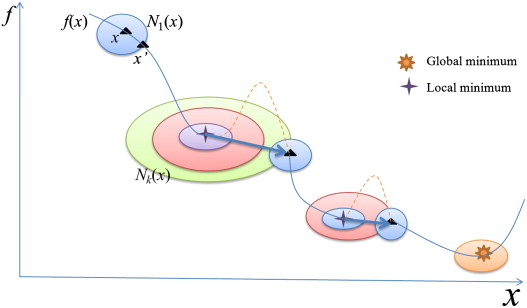
\includegraphics[width=0.4\textwidth]{../img/vns.jpg}
\end{center}
\vspace{-8mm}
\caption[Ein echter Raidl]{Veranschaulichung der Variablen Nachbarschaftssuche. \cite{Chen}}
\vspace{-8mm}
\end{wrapfigure}

Um diesem Zustand des vollkommenen Stillstandes zu entkommen, wird, nachdem dieses lokale Optimum für alle definierten Nachbarschaften erreicht wurde, mit immer größer werdenden Kraft die Lösung ``geschüttelt''. Gemeint ist damit, dass die lokal optimale Lösung durch verschiedene Algorithmen verändert wird, welche nicht darauf abzielen, eine Lösung besser zu machen, sondern sie zunächst ein wenig, mit dem Fortschreiten der Optimierung aber auch möglichst stark zu verfremden, um einen neuen Startpunkt für das VND zu besitzen.

Veranschaulichen kann man sich das Verfahren, wenn man sich alle gültigen Lösungen als eine große Fläche vorstellt. Je nach Güte der Lösung sind einzelne Teile dieser Fläche unterschiedlich hoch, gute Lösungen bilden Senken (wenige Farben werden für die Färbung benötigt), während schlechte Lösungen Berge bilden. Das VND tendiert nun dazu, sich in einer dieser Senken festzufahren, es wurde ein lokales Optimum bezüglich sämtlicher Nachbarschaften erreicht.

Mit Hilfe des ``Schüttelns'' wird nun versucht, aus eben jenen Senken zu entkommen, um eine andere, hoffentlich tiefere Senke zu finden, also eine bessere Lösung. Nach diesem Schritt beginnt der Algorithmus nämlich wieder von vorne und sucht mit Hilfe der Nachbarschaften erneut ein lokales Optimum.

Obwohl die Variable Nachbarschaftssuche in der Theorie immer weiter laufen könnte und dabei hoffentlich immer wieder neue, bessere Lösungen erreicht, wird meist eine fixe Zeit oder eine Anzahl an Iterationen bzw.\ ``Schüttelungen'' ohne Verbesserung als Abbruchkriterium gewählt.

\begin{algorithm}
\begin{algorithmic}[1]
\State Berechne Initiallösung mit \emph{onestepCD}
\While{Terminationsbedingung \textbf{nicht} erfüllt}
\State Führe Variable Neighborhood Descent mit Best Improvement Strategie durch:
\State Nachbarschaft $l \leftarrow 1$
\While{$l \leq $ maximale Anzahl an Nachbarschaften \textbf{und} Zeitlimit nicht erreicht}
\State Führe Nachbarschaft $n_l$ aus
\If {Lösung verbessert \textbf{und} $l\neq 1$} 
\State  $l\leftarrow 1$  
\Else
\State  $l\leftarrow l + 1$
\EndIf
\EndWhile
\If{Beste Lösung verbessert \textbf{oder} $k \geq k_{\mathrm max}$}
\State $k \leftarrow k_{\mathrm start}$ 
\Else
\State $k \leftarrow k + 1$
\EndIf
\State Wähle zufällig Nachbarschaft aus und ``schüttle" Lösung mit $k$ zufälligen Zügen
\EndWhile
\State\Return Beste gefundene Lösung
\end{algorithmic}
\caption{Pseudocode der Variablen Nachbarschaftssuche}
\end{algorithm}

\section{Konstruktionsheuristiken}
\label{sec:construct}
\citet*{Li2000} beschreiben mehrere schnelle Greedy Algorithmen (es wird beim Aufbau der Lösung die lokal beste Entscheidung getroffen ohne auf das große Ganze zu achten) zur näherungsweisen Lösung des Problems. Im Vergleich der benötigten Farben schneidet dabei der Algorithmus \emph{onestepCD} am besten ab:
\subsection{onestepCD}
Zunächst werden in einem Vorverarbeitungsschritt alle Kanten aus dem Konfliktgraphen entfernt, die Knoten innerhalb eines Clusters miteinander verbinden (da für jede Kommunikation nur genau ein Kommunikationsweg gewählt wird, können sich Knoten eines Clusters nie gegenseitig stören, die entsprechenden Kanten sind daher für die Lösung des Problems irrelevant und können gelöscht werden). Danach wird für jeden Cluster der Knoten mit der geringsten Anzahl an bereits eingefärbten Nachbarknoten bestimmt, der Knoten mit der insgesamt kleinsten Anzahl wird ausgewählt. Gibt es hier mehrere gleichwertige Kandidaten, wird aus diesen der Knoten mit der größten Anzahl an noch nicht eingefärbten Nachbarknoten gewählt bzw. -- falls dies immer noch nicht eindeutig möglich ist -- der erste Knoten aus diesen Kandidaten. Nachdem nun ein Knoten als Repräsentant für seinen Cluster bestimmt und ihm die klei\-nst\-mö\-gliche Farbe zugewiesen wurde, werden alle anderen Knoten, die sich im selben Cluster befinden, gelöscht. Der Prozess wird solange fortgeführt, bis die Repräsentanten aller Cluster gewählt und eingefärbt sind.

\subsection{PILOT}

Bessere Ergebnisse als die einer naiven Konstruktionsheuristik wie \textit{onestepCD} liefern häufig Varianten der gleichen Verfahren nach dem PILOT-Schema. Hier  wird grundsätzlich nach den Entscheidungskriterien von \textit{onestepCD} verfahren um jedoch nicht nur einen, sondern mehrere Knoten auszuwählen. Diese werden dann jeweils fixiert und durch Rekursion vollständige Lösungen berechnet. Von den verschiedenen Lösungen, die auf höherer Rekursionsebene zur Verfügung stehen, kann dann die vielversprechendste, also jene mit den wenigsten Farben, herangezogen werden, um eine lokal bessere Entscheidung zu treffen.

Es entsteht also eine beschränkte Enumeration der Lösungen, was deutlich zeitintensiver als die einmalige Berechnung von \textit{onestepCD} ist, aber möglicherweise deutlich bessere Ergebnisse liefert.

\begin{figure}
	\centering
	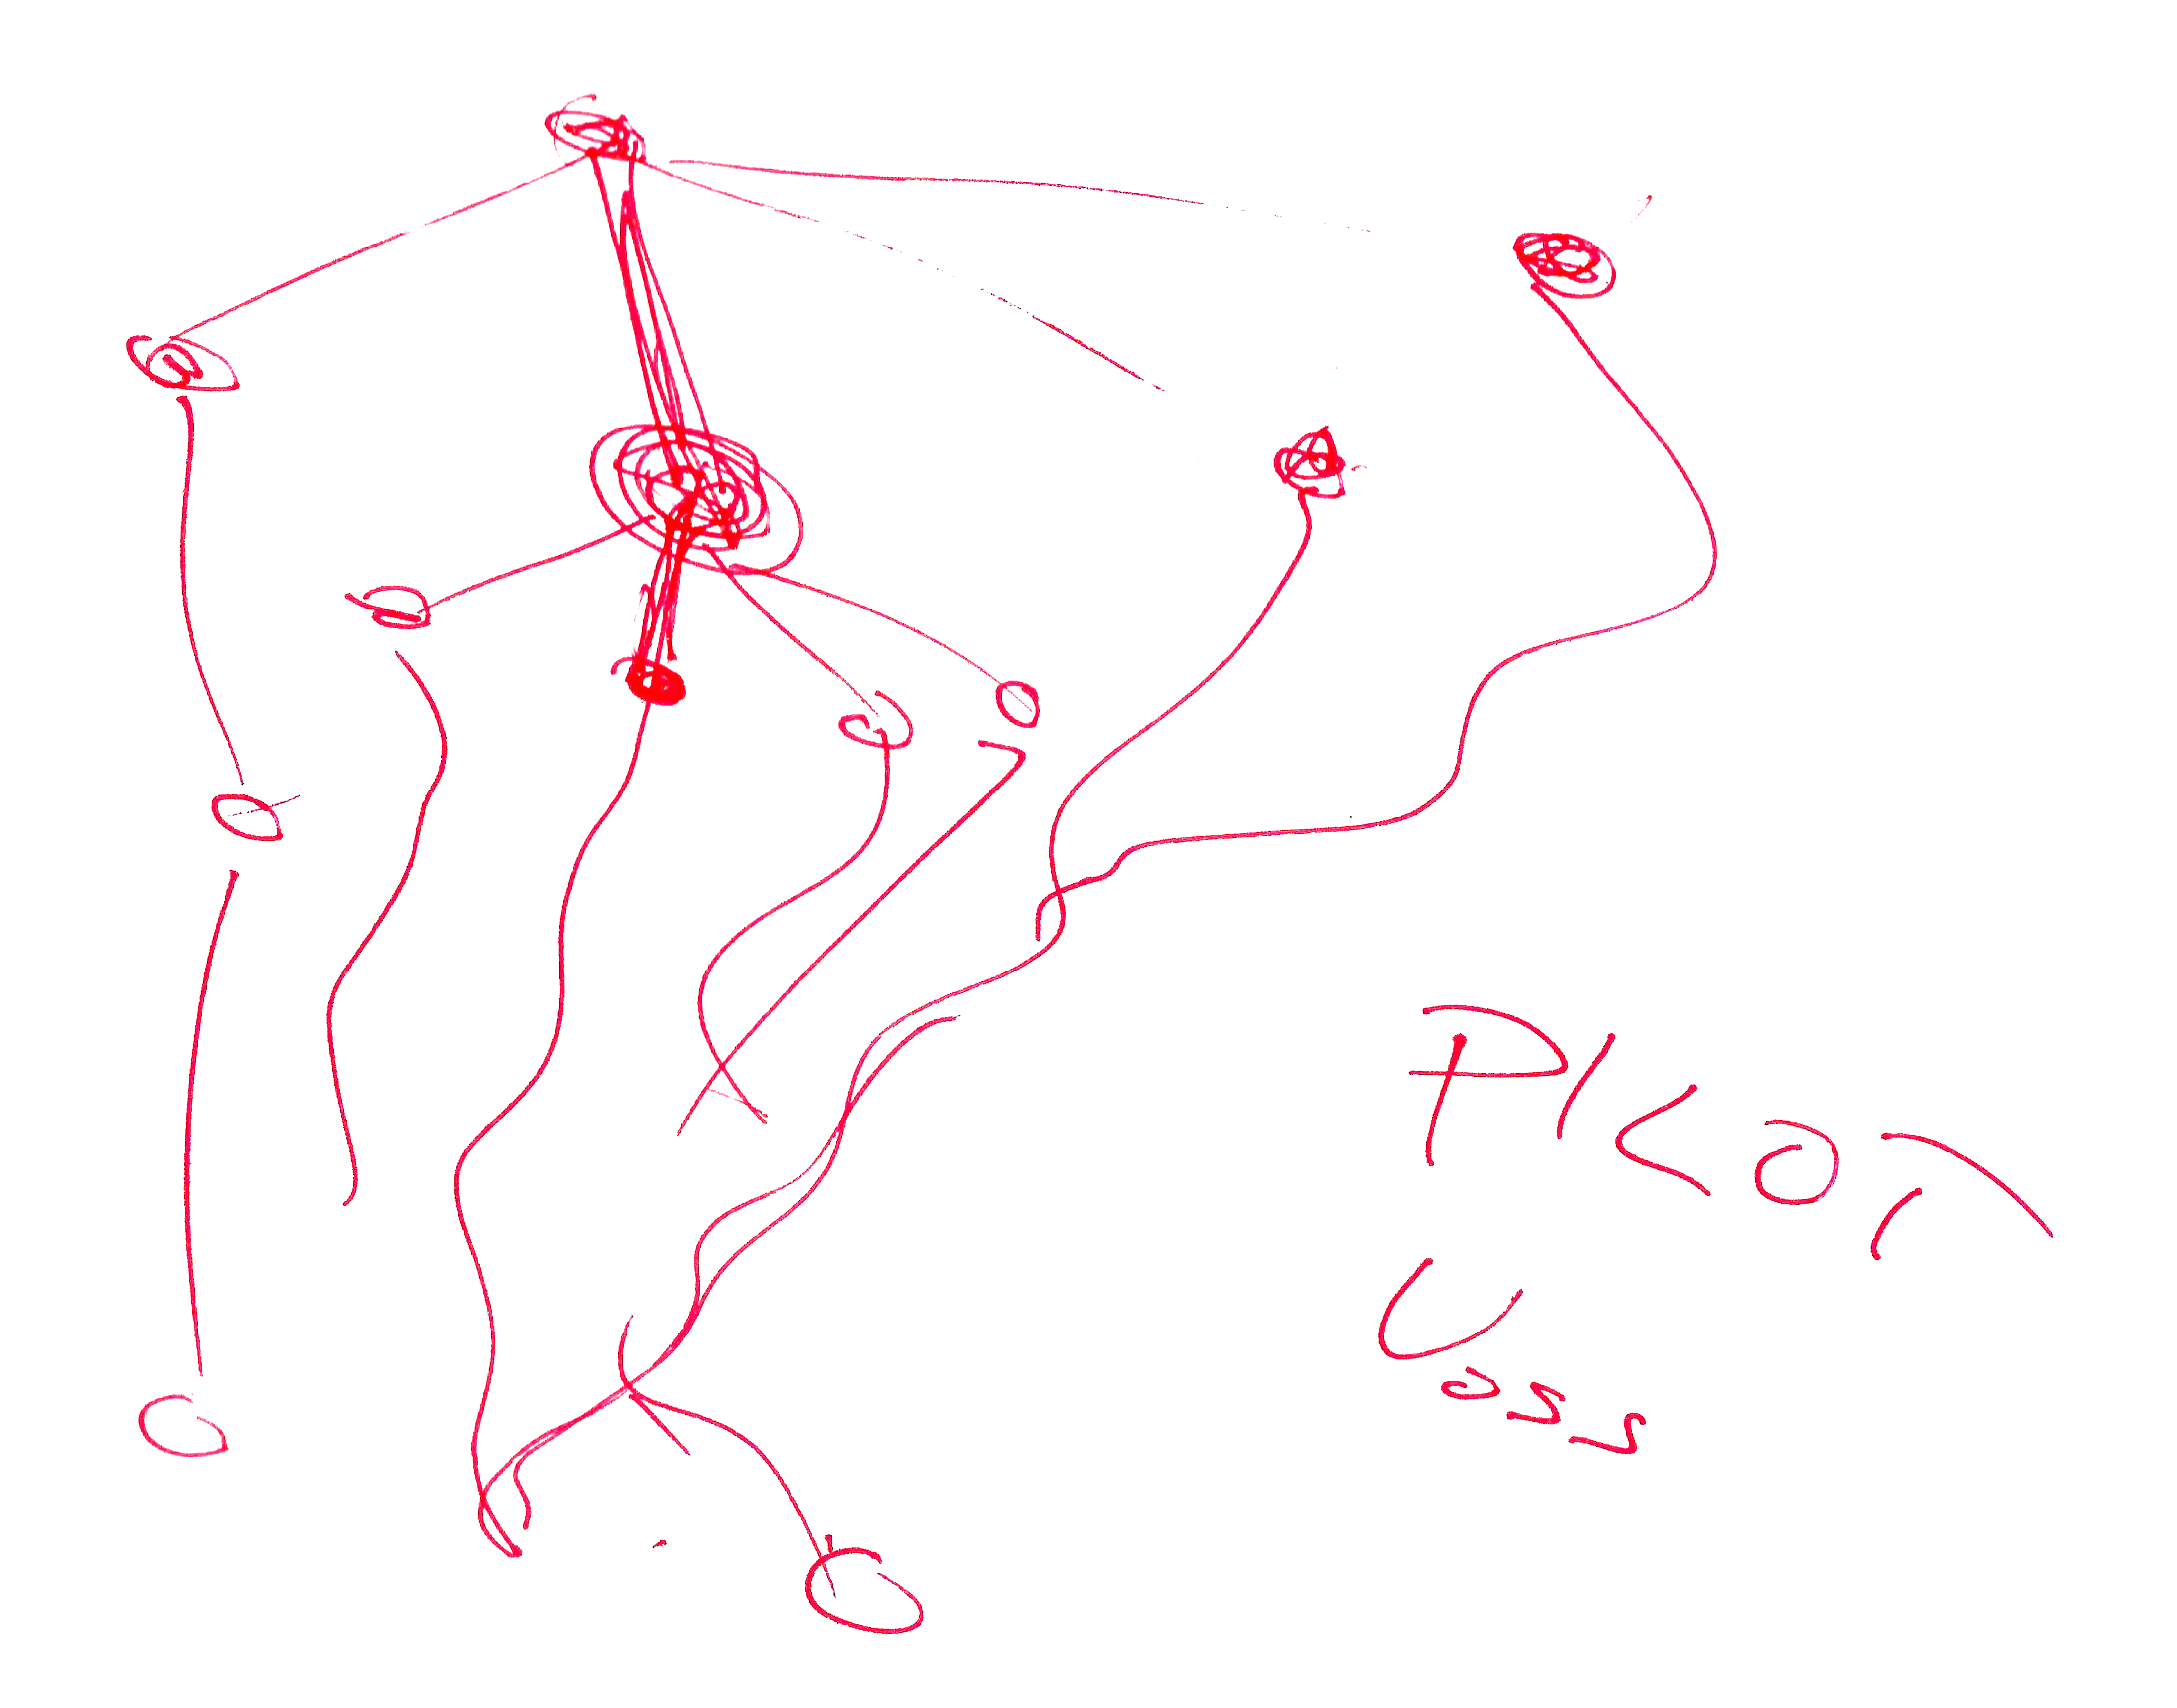
\includegraphics[width=0.7\textwidth]{../img/pilot}
	\caption{Anschauliche Darstellung des PILOT-Verfahrens}
	\label{fig:pilot}
\end{figure}

\section{Nachbarschaften}
\label{sec:neigh}
Wie bereits beschrieben handelt es sich bei Nachbarschaften um einzelne Algorithmen die versuchen, eine gültige Lösung in eine andere, bessere Lösung durch eine relativ kleine Änderung umzuwandeln. Wir haben uns zunächst auf die drei Nachbarschaften \emph{changeColor}, \emph{changeNode} und \emph{DSATUR} konzentriert, wobei weitere Nachbarschaften noch zur Diskussion stehen.

Jede Nachbarschaft bietet auch eine Methode an, eine Lösung zu ``schütteln'', welche ähnlich abläuft wie die Methode zur Suche des jeweiligen lokalen Optimums, allerdings ohne die Beschränkung ausschließlich bessere Ergebnisse zurückliefern zu müssen.

\subsection{ChangeColor}
\label{sec:changecolor}
Bei dieser sehr einfachen Nachbarschaft, die von der Tabu-Suche aus \citet*{Noronha2006} inspiriert ist, wird versucht, alle Knoten umzufärben, welche mit der höchsten Farbe markiert wurden. 

\subsubsection{Erster Ansatz}
Der erste Ansatz für diese Nachbarschaft arbeitete wie folgt.
Alle Knoten, welche die höchste Farbe besitzen, werden mit einer neuen zufälligen, aber natürlich kleineren, Farbe markiert. Dies führt meist unweigerlich zu Konflikten zwischen verbundenen Knoten im Konfliktgraph, d.h.\ zu benachbarten Knoten mit gleicher Farbe. 

Um diese Konflikte zu lösen wird ein zufälliger, im Konflikt stehender Knoten ausgewählt, um ihn mit einer passenden Farbe zu füllen. Zu beachten ist hierbei die Tatsache, das diese passende Farbe kleiner sein muss als die frühere höchste Farbe, da ja eine Verbesserung (eine Reduktion der Farbenanzahl um 1) erzielt werden soll.

Sollte sich keine passende Farbe finden, wird auch dieser im Konflikt stehende Knoten mit einer zufälligen Farbe neu eingefärbt, was im Normalfall zu weiteren Konflikten führt. Es wird nun versucht, diesen gesamten Vorgang so lange zu wiederholen bis keine Konflikte mehr bestehen. 

Sollte nach einer gewissen Anzahl an Iterationen keine konfliktfreie Lösung gefunden werden, bricht \emph{ChangeColor} automatisch ab und liefert die letzte valide Lösung zurück.

\subsubsection{Zweiter Ansatz}
Da sich in Tests dieser erste Ansatz nicht bewährte, vor allem da er bei großen Probleminstanzen zu häufig zu keinem brauchbaren Ergebnis kam, wurde der Ansatz überarbeitet. Er basiert weiterhin auf der Umfärbung der
Knoten mit der höchsten Farbe, diesmal allerdings ohne eine willkürliche Auswahl an in Konflikt stehenden Knoten.

Die veränderte Heuristik ist unter Algorihtmus~\ref{psy:ChangeColor} zu finden. Jeder Knoten, welcher die höchste Farbe besitzt, wird umgefärbt. Es werden alle Farben ausprobiert, welche kleiner als
die ursprünglich höchste Farbe sind. Dann wird versucht, die adjazenten Knoten umzufärben, und zwar so, dass auch hier nicht mehr die höchste Farbe verwendet wird. Wenn keine der ausprobierten Farben eine
Verbesserung bringt, wird die Nachbarschaft abgebrochen. Konnten für alle Knoten, welche ursprünglich die höchste Farbe besaßen, eine Ersatzfarbe gefunden werden, wird die neue Lösung zurückgegeben, 
welches eine Verbesserung zum Eingabeobjekt darstellt.

\begin{algorithm}
\begin{algorithmic}[1]
\Require Solution $s$, Solution $full$
\Ensure Solution $l$
\State $l \leftarrow$ Kopie von $s$
\State $c \leftarrow maximaleFarbe(l)$
\ForAll{Knoten $v \in l.graph$ für die gilt $v.farbe = c$}
\For{Farbe $i = 0 \to c - 1$}
\State $v.farbe \leftarrow i$
\State Färbe alle adjazenten Knoten mit gleicher Farbe neu ein
\If{$maxFarbe(v.adjazenzen) < c$}
\State Beende innere Schleife  
\EndIf
\EndFor
\If{$maxFarbe(v.adjazenzen) \ge c$}
\State Stoppe Nachbarschaft ohne bessere Lösung
\EndIf
\EndFor
\State retourniere $l$
\end{algorithmic}
\caption{Pseudocode der ChangeColor-Nachbarschaft}
\label{psy:ChangeColor}
\end{algorithm}

\subsection{ChangeNode}
\label{sec:changenode}
Diese Nachbarschaft baut auf der Tatsache auf, dass man aus einem Cluster nur jeweils einen Knoten auswählen muss. 

\subsubsection{Erster Ansatz}

In einem ersten Ansatz werden wie bei \emph{ChangeColor} alle Knoten höchster Farbe ausgewählt und umgefärbt.
Nun wird wieder ein zufälliger Knoten aus den entstandenen Konflikten ausgewählt, welcher dann aber durch einen zufälligen Knoten aus dem selben Cluster ersetzt wird. An diesem Knoten wird dann ein neuer Einfärbeversuch unternommen, wobei die maximal zulässige Farbe natürlich wieder kleiner ist als die ursprünglich höchste Farbe.

Dieser Vorgang wird solange wiederholt bis alle Konflikte gelöst wurden oder zu viele Iterationen abgelaufen sind. Wurden alle Konflikte gelöst, wurde eine neue, verbesserte Lösung gefunden, ansonsten wird die Nachbarschaft abgebrochen.

\subsubsection{Zweiter Ansatz}

Bei dem ersten Ansatz dieser Nachbarschaft ergaben sich ähnliche Probleme wie beim ersten Ansatz von ChangeColor. Durch den höheren Aufwand, der durch das Tauschen von Knoten entsteht, erwies sich dieser erste Verusch der Nachbarschaft
sogar als noch unzuverlässiger als ChangeColor. Mit Hilfe dieses zweiten Ansatzes, welcher es auch in die schlussendliche Implementierung schaffte, konnten verlässlicher und vor allem schneller Ergebnisse erzielt werden.

Die schlussendliche Variante der Nachbarschaft ist unter Algorithmus~\ref{psy:ChangeNode} zu finden. Ähnlich wie bei ChangeColor wird versucht, alle Knoten mit der maximalen Farbe umzufärben. Bei diesem zweiten Ansatz wird dies versucht, indem
ein Knoten mit maximaler Farbe gegen einen anderen Knoten ausgetauscht wird. Dieser Austauschknoten muss natürlich auch Vertreter der selben Partition sein. Dieser Knoten wird dann versucht ganz normal
neu einzufärben. Sollte die Neueinfärbung mit einer Farbe niedriger als der bisher maximalen Farbe erfolgen, wird nach weiteren Knoten maximaler Farbe gesucht. Sollte der Algorithmus nicht in der Lage sein, einen
passenden Ersatzknoten zu finden, welcher die Anzahl an verwendeten Farben verringert, bricht die Nachbarschaft ohne Verbesserung ab.

\begin{algorithm}
\begin{algorithmic}[1]
\Require Solution $s$, Solution $full$
\Ensure Solution $l$
\State $l \leftarrow$ Kopie von $s$
\State $c \leftarrow maximaleFarbe(l)$
\ForAll{Knoten $v \in l.graph$ für die gilt $v.farbe = c$}
\ForAll{Knoten $a \in full.graph$ für die gilt $a.partition = v.partition \wedge a \neq v$}
\State Tausche Knoten $v$ mit Knoten $a$ in Solution $l$
\State Färbe Knoten $a$ mit minimal möglicher Farbe ein
\If{$a.farbe < c$}
\State Beende innere Schleife
\EndIf
\EndFor
\If{$a \ge c$}
\State Stoppe Nachbarschaft ohne bessere Lösung
\EndIf
\EndFor
\State retourniere $l$
\end{algorithmic}
\caption{Pseudocode der ChangeNode-Nachbarschaft}
\label{psy:ChangeNode}
\end{algorithm}

\subsection{DSATUR}
\label{sec:dsatur}
Diese Nachbarschaft reduziert das Graph Partition Coloring Problem auf das normale Graph Coloring Problem ohne Clusterung der Knoten, indem die aktuell gewählten Repräsentanten fixiert werden und dieses so vereinfachte Problem (das allerdings immer noch NP-hart ist) wird nun mit folgendem Greedy Ansatz näherungsweise gelöst:

\begin{enumerate}
    \item Finde den (noch nicht eingefärbten) Repräsentanten mit der größten Anzahl an eingefärbten Nachbarn (engl.\ \textit{Degree Saturation}).
    \item Bei Gleichstand: Wähle den Knoten mit der größten Anzahl an nicht eingefärbten Nachbarn.
    \item Bei Gleichstand wähle den ersten Knoten in lexikographischer Abfolge.
    \item Weise dem gewählten Knoten die kleinste mögliche Farbe zu.
    \item Wiederhole, bis die Repräsentanten aller Cluster eingefärbt wurden.
\end{enumerate}

\begin{algorithm}
\begin{algorithmic}[1]
\State Lösche die aktuelle Färbung
\State Sei $t$ der ausgewählte Knoten
\State Sei $D$ die maximale Saturation
\State Sei $B$ die maximale Anzahl an nicht eingefärbten Nachbarn
\State Sei $C$ die beste Färbung
\For{$i$ = 0,\ \ldots,\ k}
\State $D \leftarrow -1$
\State $B \leftarrow -1$
\State $C \leftarrow -1$
\State $t \leftarrow $ undefiniert
\ForAll{$v \in V'$}
\If{Partition von $v$ ist eingefärbt}
\State Überspringe diesen Knoten
\Else
\State $c\leftarrow$ kleinstmögliche Färbung von $v$
\State $d\leftarrow$ Anzahl an eingefärbten Nachbarn von $v$ (\textit{Degree Saturation})
\If{$d < D$}
\State Überspringe diesen Knoten
\EndIf
\State $b\leftarrow$ Anzahl an nicht eingefärbten Nachbarn von $v$ ($deg(v) - d$)
\If{$d = D \wedge b \leq B$}
\State Überspringe diesen Knoten
\EndIf
\State Wähle $v$ als besten Kandidaten, zum jetzt Einfärben:
\State $D \leftarrow d$
\State $B \leftarrow b$
\State $C \leftarrow c$
\State $t \leftarrow v$
\EndIf
\EndFor
\State Färbe $t$ mit $C$.
\EndFor
\end{algorithmic}
\caption{Pseudocode der Nachbarschaft DSATUR}
\end{algorithm}

\subsection{ChangeAll}
\label{sec:changeall}
Bei der Nachbarschaft ChangeAll handelt es sich um eine Kombination aus den beiden Nachbarschaften ChangeColor und ChangeNode. Beide Ansätze werden kombiniert, um ihre einzelnen Stärken gemeinsam auspielen
zu können. In Tests mit großen und kleinen Probleminstanzen zeigte sich, das ChangeAll zu Verbesserungen führt, welche weder von ChangeNode noch von ChangeColor vorgenommen wurden.

Der Pseudocode ist unter Algorithmus~\ref{psy:ChangeAll} zu finden. Zuerst wird die bei ChangeNode nach einem neuen Knoten gesucht, welcher einen anderen Knoten mit höchster Farbe ersetzen soll. Dann wird
allerdings wie bei ChangeColor dieser neue Knoten in verschiedenen Einfärbungen ausprobiert. Sollte eine dieser Kombinationen aus Knotenauswahl und Farben eine Verbesserung darstellen werden weitere Knoten
mit maximaler Farbe gesucht. Sollte keine Verbesserung gefunden werden, bricht die Nachbarschaft ohne Ergebnis ab.

\begin{algorithm}
\begin{algorithmic}[1]
\Require Solution $s$, Solution $full$
\Ensure Solution $l$
\State $l \leftarrow$ Kopie von $s$
\State $c \leftarrow maximaleFarbe(l)$
\ForAll{Knoten $v \in l.graph$ für die gilt $v.farbe = c$}
\ForAll{Knoten $a \in full.graph$ für die gilt $a.partition = v.partition \wedge a \neq v$}
\State Tausche Knoten $v$ mit Knoten $a$ in Solution $l$
\For{Farbe $i = 0 \to c - 1$}
\State $a.farbe \leftarrow i$
\State Färbe alle adjazenten Knoten mit gleicher Farbe neu ein
\If{$maxFarbe(a.adjazenzen) < c$}
\State Beende innerste Schleife
\EndIf
\EndFor
\If{$maxFarbe(a.adjazenzen) < c$}
\State Beende mittlere Schleife
\EndIf
\EndFor
\If{$maxFarbe(a.adjazenzen) \ge c$}
\State Stoppe Nachbarschaft ohne bessere Lösung
\EndIf
\EndFor
\State retourniere $l$
\end{algorithmic}
\caption{Pseudocode der ChangeAll-Nachbarschaft}
\label{psy:ChangeAll}
\end{algorithm}

\chapter{Implementierung}
%TODO: sec:ansatz
Für die Implementierung des in Abschnitt \ref{sec:ansatz} vorgeschlagenen Lösungsansatzes, wurde eine möglichst flexible Struktur des Programmes verwendet. Wie in Abschnitt \ref{sec:cpp} begründet, wurde
als Implementationssprache C++ gewählt. Durch den Einsatz von C++ kann ein einfach erweiterbares Programmgerüst geschrieben werden, welches es erlaubt, schnell und ohne großen Aufwand mehrere Nachbarschaften
für die VNS zu implementieren. 

Um diese flexible Struktur zu ermöglichen wurde das Programm in vier unabhängige Bereiche aufgeteilt, welche durch eine einzelne Startroutine zusammengehalten werden. Diese Bereiche können grob als Parser, 
Konstruktionsheuristik, Variable Nachbarschaftssuche, und Nachbarschaften zusammengefasst werden. Hinzu kommt die sogenannte Solution, eine eigene Klasse um eine Lösung sowohl zu speichern, aber auch um Möglichkeiten
anzubieten, eine bestehende Lösung zu verändern. Diese einzelnen Bereiche sollen im folgenden Abschnitt ausführlich besprochen werden.

\section{Solution}
Bei Solution handelt es sich um die Basisklasse für alle weiteren Operationen. Sie speichert sowohl den Graphen, von dem bei der Lösung ausgegangen wird, als auch die Lösung selbst, mit konkret verteilten Farben
für einzelne Partitionen. Außerdem stellt Solution Methoden bereit, um Veränderungen an Lösungen vorzunehmen, wie sie etwa von den Nachbarschaften gebraucht werden, um einzelne Knoten umzufärben, oder zu ersetzen.
Außerdem besitzt Solution mehrere Methoden, einen Problemgraphen aus einer Datei auszulesen, und diesen wiederum in einem Solution-Objekt zu speichern. Diese Methoden zum Einlesen von Dateien werden genauer 
in Abschnitt \ref{sec:parser} besprochen.

\singlespacing
\lstset{style=customc}
\begin{lstlisting}[caption={Signatur der Solutionklasse},label=lst:solution]
class Solution {
   public:
      Solution();
      Solution(Solution *s);
      ~Solution();
      
      void requestDeepCopy();

      Graph *g;
      int numParts;
      int *partition;
      std::vector<Vertex> *partNodes;
      int colorsUsed;
      int *representatives;
      int *copyCounter;
      
      int getPartition(Vertex v);
      unsigned int getOriginalId(Vertex v);
      int getPartitionColor(Vertex v);
      int getColorDegree(Vertex v);
      
      int minPossibleColor(Vertex v);
      boost::tuple<int, int> getColorDegreeAndMinColor(Vertex v);
      bool isPartitionColored(Vertex v);
      
      void setOriginalId(Vertex v, int id);
      void setPartitionColor(Vertex v, int color);
      
      void print(std::ostream& out);
      std::string toString();
      
      static Solution* fromColStream(std::istream& in);
      static Solution* fromColBStream(std::istream& in);
      static Solution* fromPcpStream(std::istream& in);
      
      void addVertex(int part, Vertex id);
      void removeVertex(Vertex id);
      void addEdge(Vertex v1, Vertex v2);
      void replaceVertex(Vertex toR, Vertex rep, Solution& full);
      
      #ifdef ubigraph
      void redraw();
      void redraw(int shift);
      void prepareUbigraph();
      #endif
      
   private:
      boost::property_map<Graph, boost::vertex_index1_t>::type partitionMap;
      boost::property_map<Graph, boost::vertex_index2_t>::type idMap;
};
\end{lstlisting}
\setstretch{1.5}

Besonders interessant bei der Solution-Klasse ist die automatisch bereitgestellte Kopiermechanik. Einer der besonderen Eigenschaften von C++ ist es, für jede Klasse automatisch einen sogenannten Kopierkonstruktor
bereitzustellen, welcher als Parameter ein Objekt des selben Types entgegennimmt, und dieses kopiert. Da im Falle einer Lösung aber nicht immer alle Daten kopiert werden müssen, wurde in dieser Arbeit eine
eigene Kopiermechanik implementiert. Wie in Listing \ref{lst:copy} zu sehen ist, wird ein Großteil der Referenzdatentypen direkt übernommen, da diese häufig garnicht verändert werden. 

Das Kopieren einer Lösung kommt vor Allem bei den verschieden Nachbarschaften zum Einsatz. Eine bestehende Lösung soll verändert werden, ohne, dass die Information der Ausgangslösung verloren geht. Also wird
die bestehende Lösung kopiert, und die Veränderungen nur auf der neuen Lösung ausgeführt. Da viele der Nachbarschaften darauf basieren, dass ausschließlich die Lösungsfarben verändert werden, kann zum Beispiel, 
anstatt den gesamten Graphen zu kopieren, eine Referenz auf den alten Graphen aufrecht erhalten werden. Selbiges gilt natürlich auch für alle direkt mit dem Graph in Verbindung stehenden Datenspeichern. 

\singlespacing
\begin{lstlisting}[caption={Der Kopierkonstruktor der Solutionklasse},label={lst:copy}]
Solution::Solution(Solution *toCopy) {
   this->partNodes = NULL;
   this->g = toCopy->g;
   this->representatives = toCopy->representatives;
   this->partitionMap = get(vertex_index1_t(), *this->g);
   this->idMap = get(vertex_index2_t(), *this->g); 
   // Copy reference counter and increment to track references
   this->copyCounter = toCopy->copyCounter;
   *this->copyCounter += 1;  
   
   this->numParts = toCopy->numParts;
   this->colorsUsed = toCopy->colorsUsed;

   
   this->partition = new int[this->numParts];
   for (int i = 0; i < this->numParts; i++) {
      this->partition[i] = toCopy->partition[i];
   }
}
\end{lstlisting}
\setstretch{1.5}

Nun könnten aber Probleme entstehen. Zum einen, wenn eine Nachbarschaft beispielsweise Knoten aus dem zu Grunde liegenden Graphen austauscht, um eine bessere Lösung zu erhalten. Da durch das unechte Kopieren
der in einem Solutionobjekt referenzierte Graph auch bei anderen Lösungen zum Einsatz kommt, würde eine Veränderung auf einem Graphen, zu Veränderungen und aller Wahrscheinlichkeit nach zu Fehlern in alternativen
Lösungen führen, welche dann unweigerlich unzulässige Ergebnisse zur Folge hätten. Daher kann mit der Methode \texttt{requestDeepCopy} eine vollständige Kopie des Solutionobjektes angefordert werden. In dieser
Methode werden dann alle verbleibenden Fremdreferenzen nocheinmal kopiert, und in eigens für das anfragende Solutionobjekt reservierte Speicherbereiche geschrieben.

Ein anderes Problem entsteht beim Aufräumen von Objekten. Sollte durch das Löschen eines Solutionobjektes auch dessen referenzierter Graph verschwinden, würde das zu Speicherfehlern bei anderen Objekten führen, 
welche auf den selben Graphen zeigen. Daher wurde der Destruktor, welcher zum Aufräumen eines Objektes aufgerufen wird, überschrieben, und löscht nun nur noch referenzierte Objekte, wenn kein anderes Objekt
mehr Referenzen auf das selbe Objekt hält. Um dies zu ermöglichen wird von allen Solutionobjekten, welche auf den selben Graphen referenzieren ein Counter referenziert, welcher die Anzahl der
Verweise auf den selben Graphen mitzählt. So lange dieser Zähler über eins ist, wird kein Objekt gelöscht. Wird nun der Destruktor eines Solutionobjektes aufgerufen, überprüft dieser, ob er die letzte
Referenz auf diese Objekte hält. Wenn ja, löscht er diese und seine eigenen Referenzen, wenn nicht, löscht er wiederum nur seine eigenen Referenzen und vermindert den Zähler um eins.

\subsection{StoredSolution}
Um eine einzelne Lösung von einer anderen zu unterscheiden, sind zwei Informationen notwendig: die Auswahl der Repräsentanten, und die Auswahl 
an Farben. Mit diesen beiden Informationen, und dem Ausgangsgraphen, aus dem die Lösung berechnet wurde, ist eine Lösung eindeutig rekonstruierbar.
Umzu verhindern, dass die VNS-Schleife immer wieder auf die selben Lösungen kommt, ohne echte Verbesserungen zu erzielen, werden alle neuen, verbesserten
Lösungen komprimiert gespeichert. 

Zur komprimierten Speicherung wurde eine eigene Datenstruktur definiert, welche eben nur jene oben erwähnten Informationen abspeichert. 
Dazu werden zwei Arrays verwendet, welche einerseits die für einzelne Partitionen verwendeten Farben, andererseits aber auch die 
eindeutige Identifikationsnummern der Repräsentanten abspeichern. Um eine Solution einfach in solch eine StoredSolution umzuwandeln, wurde
ein Konstruktor definiert, welcher ein klassisches Solutionobjekt übernimmt. 

\singlespacing
\begin{lstlisting}[caption={Die Signatur von StoredSolution},label={lst:stored}]
struct StoredSolution {
   StoredSolution(Solution& toStore);
   ~StoredSolution();
   
   int n;
   
   int *colors;
   int *representatives;
   
   std::string toString();
};
\end{lstlisting}
\setstretch{1.5}

Für den schnelle Zuordnung einer neuen Lösung zu den bestehenden Lösungen wird eine Hashmap-Datenstruktur verwendet. Durch die Verwendung einer
Hashmap ist eine quasi sofortige Zuordnung einer Lösung zu dem entsprechenden Platz in der Hashmap möglich. Sollte eine Lösung schon einmal 
aufgekommen sein, wird dieser Lösungsstrang verworfen, da er nicht zu neuen Lösungen führen würde. Die Implementation der Hashmap wird von 
Boost, beschrieben im Abschnitt \ref{sec:boost}, bereitgestellt. Um die Hashmap zu betreiben sind außerdem noch eine Methode zur Hashberechnung,
sowie eine Methode zum Vergleich zweier gespeicherten Solutions notwendig. Der Hash für ein StoredSolutionobjekt wird aus den gesammelten Werten
der beiden internen Arrays berechnet, während für die Vergleichsmethode die beiden Arrays Wert für Wert verglichen werden. Die von Boost 
bereitgestellte Hashmap verwendet bei gleichen Hashwerten aber unterschiedlichen Lösungen eine einfache Liste, um die Ergebnisse zu speichern.

\section{Parser}
\label{sec:parser}

Damit erzielte Ergebnisse mit älteren Programmversionen, aber auch mit anderen Lösungsansätzen für das PCP verglichen werden können, ist es von
Vorteil, immer wieder die selbe Eingabe zu verwenden. Außerdem bietet sich eine solche Möglichkeit an, wenn, wie in dieser Arbeit ein Zufallsfaktor
zu einer Verbesserung der Lösung führen kann. Durch immer wieder gleiche Eingaben kann ein direkter Vergleich auch zwischen unterschiedlich
parametrisierten Programminstanzen angestellt werden.

Es gibt mehrere Dateiformate, mit denen Probleminstanzen des PCP abgespeichert werden können. In dieser Arbeit wurde vor Allem auf jenes
Format Wert gelegt, in dem auch die meisten Testinstanzen der einschlägigen Literatur vorliegen. Allerdings wurde im Zuge von ausgeweiteten 
Testungen auch ein zweites Format zum einlesen eines Problemgraphen implementiert. 

Eine \texttt{.pcp}-Datei ist eine einfache Textdatei, welche allerdings nach einer bestimmten Struktur aufgebaut ist. Die aller erste Zeile
einer solchen Datei besteht aus 3 Zahlen, welche jeweils durch ein Leerzeichen getrennt sind. Diese 3 Zahlen stehen für die Anzahl der Knoten, 
die Anzahl der Kanten, und die Anzahl der Partition im Problemgraph, genau in jener Reihenfolge. Nun folgen \textit{n} Zeilen an Zahlen, mit 
genau einer Zahl pro Zeile, wobei \textit{n} die Anzahl an Knoten ist. Diese Zahlen stehen für die Partitionen, denen die Knoten zugeordnet werden.
Die erste Zeile beinhaltet also die Partition des ersten Knotens, die zweite Zeile die des zweiten Knotens und so weiter. Zu letzt folgen noch
\textit{m} Zeilen mit jeweils einem Zahlenpaar, welche die Kanten zwischen den Knoten definieren, wobei \textit{m} der Anzahl an Kanten insgesamt
entspricht.

\singlespacing
\begin{lstlisting}[caption={Eine einfache \textit{.pcp}-Beispieldatei},label={lst:pcp}]
4 5 2
0
1
1
0
0 1
0 2
1 2
1 3
2 3
\end{lstlisting}
\setstretch{1.5}

Der Parser, welcher eine solche Datei einliest, ist in die Klasse Solution eingearbeitet. Die statische Methode \texttt{fromPcpStream} ließt eine
Datei von einem Eingabestream ein, und wandelt sie in ein Solutionobjekt mit entsprechendem Problemgraphen um. Dieses Solutiobjekt wird während
der gesamten Laufzeit des Programmes nicht verändert oder gelöscht, und dient als Ausgangspunkt der Konstruktionsheuristik, aber auch als
Referenz für Nachbarschaften, welche einzelne Knoten austauschen.

\singlespacing
\begin{lstlisting}[caption={Die Methode \texttt{fromPcpStream}, welche eine Datei im \texttt{.pcp}-Format einließt und in ein Solutionobjekt umwandelt},label={lst:frompcp}]
Solution* Solution::fromPcpStream(istream& in) {
   Solution *s = new Solution();
   
   int vertices, edges, partitions;
   cin >> vertices >> edges >> partitions;
   
   if (DEBUG_LEVEL > 3) {
      cout << "Reading " << vertices << " vertices, " << edges;
      cout << " edges and " << partitions << " partitons ..." << endl;
   }
   
   // Initialize the solution to the read parameters
   s->partition = new int[partitions];
   s->representatives = new int[partitions];
   s->partNodes = new vector<Vertex>[partitions];
   s->numParts = partitions;
   s->colorsUsed = partitions;
   
   #ifdef ubigraph
   s->prepareUbigraph();
   #endif

   // Read partition info and store it into the property map, do the 
   // same for the "original" vertexID, so they can be compared on 
   // all graph
   int i, part;
   for (i = 0; i < vertices; i++) {
      cin >> part;
      s->addVertex(part, i);
      
      if (DEBUG_LEVEL > 3)
         cout << "Added vertex " << i << " to partition " << part << "." << endl;
   }

   // Read the input for edges between to vertices and add them to 
   // the solution graph
   for (i = 0; i < edges; i++) {
      int source, target;
      cin >> source >> target;

      if (DEBUG_LEVEL > 3) {
         cout << "Added edge (" << source << "|" << target << ")" << endl;
      }
      s->addEdge(source, target);
   }
   
   if (DEBUG_LEVEL > 3)
      cout << "Parsing input finished successfully!" << endl;

   return s;
}
\end{lstlisting}
\setstretch{1.5}


\section{Konstruktionsheuristik}

\section{Variable Nachbarschaftssuche}

\section{Nachbarschaften}

\subsection{changeColor}
\subsection{changeNode}
\subsection{DSATUR}
\subsection{changeAll}


 

\section{Implementierung}
% TODO: everything 

\subsection{C++}
Als primäre Programmiersprache wurde C++ gewählt. Verschiedene Gründe sprachen für C++, unter anderem die an C angelehnte Syntax, aber
auch die gute Performance im Vergleich zu Sprachen, welche in einer Virtuellen Maschine laufen, oder gar interpretiert werden. Zu 
all diesen Gründen kam noch hinzu, dass für C++ bereits ausgezeichnete Codebibliotheken zur Verfügung stehen, welche ein schnelles
und effizientes Arbeiten ermöglichen.

Bei C++ handelt es sich um eine im Jahr 1979 von Bjanre Stroustrup entwickelte Programmiersprache, welche anfangs als \textit{C mit Klassen}
ausgelegt wurde. Über mehrere Entwicklungsschritte entwickelte sich eine Sprache, dessen Wurzeln in der Sprache C immer noch zu erkennen sind, 
dessen Möglichkeiten jene von C aber bei weitem übersteigen. 

Wie C handelt es sich bei C++ um eine statisch-typisierte Programmiersprache, das heißt der Compiler kann schon während der Übersetzung die
syntaktisch korrekte Verwendung von Datentypen sicherstellen. Dadurch können solche Überprüfungen während der Ausführung des Programmes
entfallen, was zu einer enormen Beschleunigung der Ausführung des Programmes führt. Außerdem ermöglicht es dem Entwickler Fehler mit
inkorrekt verwendeten Datentypen einfacher zu erkennen, da eine Fehlermeldung des Übersetzers eine genau Zeile angeben kann, in der 
der Fehler verursacht wird. 

Obwohl sich C++ wesentlich von C unterscheidet, ist es immer noch kompatibel mit C. Eine Stück C Code kann immer noch in C++ verwendet und
übersetzt werden. Dadurch können nicht nur Code-Bibliotheken aus dem C++-Umfeld verwendet werden, sondern auch ursprünglich für C gedachte
Bibliotheken eingebunden und verwendet werden. Da C immer noch eine der beliebtesten Programmiersprachen weltweit, und vor allem \textbf{die}
Sprache für Systemprogrammierung und performante Software ist, bedeutet diese Mitnahme der Vorteile aus der C-Welt in die Welt von C++
einen großen Vorteil bei der Programmierung.

Des Weiteren wurde C++ möglichst plattformunabhängig designt. Während manche Funktionen, welche vom Betriebssystem bereit gestellt werden, 
natürlich nicht wirklich plattformunabhängig sein können, wurde in C++ versucht, keine Funktionen oder Eigenschaften zu verwenden, welche
nur von einem bestimmten System ausgeführt werden können. Aus diesem Grund sind auch die meisten Code-Bibliotheken für C++ für die meisten
Plattformen erhältlich. 

Obwohl C++ wesentlich mehr Funktionen als C bietet, ist trotzdem noch die Anlehnung an C zu erkennen. Daher ist es auch nicht verwunderlich das C++-Programme meist nur geringfügig langsamer sind, als 
vergleichbare C-Programme. In manchen Fällen ist C++ sogar schneller als C, da der Compiler andere, und umständen bessere, Optimierungen vornehmen kann. 

\subsubsection{STL}
\label{sec:stl}
Zusätzlich zu erwähnen ist die umfangreiche \textit{Standard Template Library (STL)}, welche es inzwischen sogar fast vollständig in den 
C++-Standard gebracht hat. Bei der STL handelt es sich um eine von den meisten Compilern bereitgestellte Code-Bibliothek für häufig 
verwendete Datenstrukturen und Hilfsroutinen, welche eine wesentliche Erleichterung für jeden C++-Programmierer darstellen. Unter anderem
in der STL enthaltene Datenstrukturen sind Listen, Stacks, aber auch Iteratoren für die meisten Datenstrukturen, häufig verwendete Algorithmen
wie Quicksort, Binarysearch. Hinzu kommen vereinheitlichte Ein- und Ausgabemöglichkeiten für verschiedenste Plattformen, sowie die 
Möglichkeit der parallelen Ausführung von Software mit Hilfe von Threads.

Die STL wurde inzwischen in den Sprachstandard von C++ aufgenommen, so dass jeder standardkonforme Comipler eine Implementierung der STL inkludiert. Mit der STL hebt sich C++ stark von C ab, für 
das es keine solche allgemein einsetzbare Codebibliothek gibt. Der Preis für diese Einfachheit ist die Zeit, die ein einzelner Übersetzungsdurchgang benötigt. Da die STL stark auf die namensgebenden
\textit{Templates} setzt, welche es ermöglichen eine einzelne Datenstruktur für eine Vielzahl an Datentypen verfügbar zu machen, muss der Compiler diese \textit{Templates} zum Übersetzungszeitpunkt
auflösen, ein Vorgang, welcher einen stark negativen Einfluss auf die Übersetzungszeit hat.

\subsection{Python}
% TODO: LOLO!

\subsection{Make}
\label{sec:make}
Bei GNU make handelt es sich um ein Standardwerkzeug der Linux-Software-Entwicklung. Mit Hilfe von make kann die Übersetzung des Quellcodes in den Programmcode automatisiert werden. 
Dabei stellt make viele verschiedene Konfigurationsmöglichkeiten bereit. Unter anderem können verschiedene Compiler, aber auch verschiedene Übersetzungsmodi eingestellt werden.
Um ein schnelleres Übersetzen zu ermöglichen, werden außerdem nur jene Quellcode-Dateien neu übersetzt, welche sich seit dem letzten Mal verändert haben. 

In der Konfigurationsdatei für make, dem so genannten Makefile, können unter anderem mehrere \textit{Targets} angegeben werden, also quasi verschiedene Endprogramme, oder verschiedene
Übersetzerkonfigurationen für das selbe Programm. Zu diesen \textit{Targets} werden dann Ab\-hängig\-keiten definiert, welche bestimmen, in welcher Reihenfolge das Programm übersetzt werden 
muss. Impliziert wird durch diese Abhängigkeitsdefinition auch, wann ein Programmteil neu übersetzt werden muss. Ist eine der Abhängigkeiten einer bestimmten Enddatei jünger als die 
Enddatei selber, muss diese neu übersetzt werden. Durch eine geschickte Aufteilung des Quellcodes auf mehrere Dateien kann so eine komplette Neuübersetzung vermieden werden. 

Durch verschiedene Variablen, welche ebenfalls im Makefile spezifiziert sind, kann außerdem, ohne großen Aufwand, der Übersetzer, welcher die eigentliche Hauptaufgabe übernimmt ausgetauscht werden.
Die für diese Arbeit verwendeten Compiler werden in Abschnitt \ref{sec:compiler} besprochen. Vereinfacht wird dies durch die beinahe gleiche Befehlssyntax, die von beiden Compilern verwendet wird.
Hinzu kommt die Tatsache, dass die von den beiden Compilern erzeugten Dateiformate miteinander kompatibel sind, so dass auch uneinheitlicher Übersetzung mit immer wieder wechselnden Übersetzern
keine Fehler entstehen.

Außerdem hilfreich ist, dass make auch Skripte oder kleinere Kommandos automatisch aus\-füh\-ren kann. Häufig verwendet ist etwa die Routine zur Bereinigung des Programmverzeichnisses von bei der
Übersetzung entstandenen temporären Dateien, die nachher nicht mehr benötigt wurden. Auch nützlich ist etwa die vollständige Entfernung jeder Spur einer Compilierung, um eine gänzlich neue
Übersetzung einzuleiten. Auch kann mit Hilfe von solchen Skripten das entstandene Programm nach Übersetzung automatisch auf eine Testmaschine geschickt werden, um die korrekte Funktion
des Programmes zu verifizieren.

\subsection{Compiler}
\label{sec:compiler}
Der Compiler, oder Übersetzer, ist dafür verantwortlich, ein Programm von einer Quellsprache, in eine Zielsprache zu übersetzen. Im Falle dieser Arbeit war die Quellsprache C++, und die
Zielsprache die Maschinensprache des Prozessors, also ein x86-Assembly. Übersetzer sind außerordentlich komplexe Stücke an Software, welche nicht einfach die Befehle eines Programmierers eins zu
eins übernehmen, sondern auch noch Optimierungen vornehmen, um eine beschleunigte Programmausführung zu ermöglichen. Da dieser Vorgang sehr zeitaufwendig sein kann, ist es wichtig, Werkzeuge wie
das in Abschnitt \ref{sec:make} besprochene make einzusetzen, um eine vollständige Neuübersetzung bei nur marginalen Änderungen im Quellcode zu verhindern. 

Da C++ eine besonders komplexe Sprache, mit vielen verschiedenen, aufwendigen Funktionen und Sprachbesonderheiten ist, ist die Übersetzung eines C++-Quellcodes besonders aufwendig. Selbst kleinere
C++-Programme können schon mehrere Minuten zum vollständigen Übersetzen brauchen. Dies gilt insbesondere für Quellcode, welche die C++-Funktion der so genannten \textit{Templates} benützt. \textit{Templates}
erlauben es, neben anderen Dingen, eine allgemeine Datenstruktur für viele verschiedene Datentypen zu programmieren, ohne eine konkrete Implementation für einen bestimmten Datentyp notwendig zu machen.
Da auch mehrere \textit{Templates} geschachtelt werden können, und dies alles zum Zeitpunkt der Übersetzung expandiert werden muss, um schließlich übersetzt werden zu können, kann bei starker Verwendung
von solchen Funktionen die Geschwindigkeit der Übersetzung stark beeinträchtigt werden.

Um diese Probleme mit \textit{Templates} elegant zu umgehen, gibt es \textit{Precompiled Headers}. Normalerweise werden Header-Dateien, welche allgemeine Deklarationen von Klassen, verwendeten Datentypen
und ähnliches enthalten, zum Übersetzungszeitpunkt in den C++-Quellcode, welcher übersetzt werden soll, komplett kopiert, und diese Gesamteinheit als eine Über\-setzungs\-einheit angesehen. Dadurch muss, sollte
sich ein Teil der Definitionen innerhalb des C++-Codes ändern, auch die Definition neu übersetzt werden. Mit \textit{Precompiled Headers} wird dieses Problem gelöst, in dem schon der Header als zu übersetzende
Einheit angesehen wird, und als vom eigentlichen Quelltext abgetrennte Einheit angesehen wird. Der Header, welcher ja unter anderem auch die Deklarationen für \textit{Templates} enthält, muss nur noch
übersetzt werden, wenn sich in seinem eigenen Code etwas ändert. Dadurch können die eigentlichen Programmabschnitte, welche in normalen C++-Quelldateien zu finden sind, wesentlich schneller
compiliert werden, ohne auf die Vorteile von \textit{Templates} zu verzichten.


\subsubsection{GCC}
GCC, oder auch GNU Compiler Collection, ist ein Sammlung an Übersetzern welche alle unter der Open-Source-Lizenz GPL veröffentlich wurden. GCC wird häufig als der Standard-Compiler unter Linux angesehen,
und erfreut sich immer noch großer Beliebtheit. Die Sammlung unterstützt viele verschiedene Sprachen, unter ihnen auch C++, sowie mehrere verschiedene Standards einzelner Sprachen. Auf Grund seiner
ausgiebigen Testung und Erprobung im alltäglichen Einsatz, und nicht zuletzt seiner freien Verfügbarkeit, bleibt GCC immer noch einer beliebtesten Compiler weltweit. Dabei ist die Sammlung verschiedener
Compiler vor allem im Umfeld der Softwareentwicklung für Linux beliebt, er kann aber auch für die Entwicklung auf Windows oder anderen Betriebssystemen eingesetzt werden.

Ein wichtiges Merkmal von \textit{g++}, dem C++-Compiler in der Sammlung von GCC, ist sein evolutionäres Wachstum seit seiner Entstehung. Da C++ mit den Jahren immer wieder leicht angepasst und um Funktionen
erweitert wurde, musste sich auch GCC anpassen, um mit diesen Änderungen Schritt zu halten. Daher wurden im Laufe der Jahre immer wieder Teile von \textit{g++} neu geschrieben, umgebaut, oder gänzlich
neue Funktionen hinzuprogrammiert. Daraus ergeben sich aber Konsequenzen, welche unter anderem die Code-Qualität negativ beeinträchtigen. Zwar Implementiert GCC auch den neuesten Standard von C++, allerdings
ist die Qualität der Implementierung sehr stark abhängig von dem Alter des entsprechenden Standards. Während ältere Standards bereits ausgiebig getestet wurden, ist bei neuen Standards eine korrekte 
Implementierung nicht immer gegeben. 

Auf Grund dieser gewachsenen Struktur von GCC ist der \textit{g++}-Compiler nicht der schnelleste Vertreter seiner Art. Vor allem die Übersetzung von Headern nimmt mit der GCC mehr Zeit in Anspruch als
bei der Konkurrenz. Wie viele andere Compiler unterstützt auch \textit{g++} die übersetzung von Header-Dateien in \textit{Precompiled Headers}. Dazu wird ein GCC-eigene Format verwendet, und \textit{g++} sucht bei einer
späteren Einbindung eines Headers in den Quellcode nach einer gleichnamigen Datei mit der Endung ``.gch''. Die Verwendung von solchen \textit{Precompiled Headers} beschleunigt die Übersetzung ungemein, 
obwohl die Übersetzung des Headers selber einige Zeit in Anspruch nimmt. Die für diese Arbeit verwendeten \textit{Precompiled Headers} bewegeten sich in der Größenordnung von knapp über 100 Megabyte, 
eine erstaunliche Datenmenge für eine einzige Übersetzungseinheit. Diese Datenmengen sind vor allem den \textit{Templates} geschuldet, welche während ihrer Expansion wesentlich an Speicherbedarf zunehmen.

\subsubsection{clang}
Bei clang handelt es sich um einen neuen Konkurrenten für GCC am Markt der Open-Source-Compiler. Wie bei GCC handelt es sich bei clang nicht um einen einzelnen Übersetzer für eine einzelne Programmiersprache,
sondern viel mehr um eine Sammlung an Übersetzern für vor allem mit C verwandten Sprachen wie C++ und Objective-C. Anders als GCC ist clang aber nicht über mehrere Jahrzehnte angewachsen, das Projekt
startete erst vor wenigen Jahren. Auch baut clang nicht von Grund auf einen neuen Compiler, sondern benützt das Rahmenwerk der LLVM, der \textit{Low Level Virtual Machine}. LLVM ist ein Projekt, welches
mit dem Ziel gestartet wurde, Techniken des Just-in-Time-Übersetzens zu den Sprachen C und anderen Low-Level-Sprachen zu bringen. Dazu wird eine eindeutige Zwischensprache, zwischen Quell- und Zielsprache
definiert, welche dann von LLVM optimiert werden kann. Diese Technik, welche ursprünglich zur Laufzeit eines Programmes zum Einsatz kommen sollte, wurde schließlich so adaptiert, um einen Compiler von
eben jener Zwischensprache zur Zielsprache zu bilden. 

Clang wurde nun mit dem Ziel geschaffen, einen sauber programmierten, standard-konformen Compiler für den produktiven Einsatz zu schaffen. Dazu wurde zunächst vor allem auf die Entwicklung eines C-Frontends
Wert gelegt. Als das C-Frontend einen arbeitsfähigen Zustand erreichte, beschloss man, auch C++ als Quellsprache mit einzuschließen. Da C++ eine sehr umfangreiche Sprache mit vielen verschiedenen Spracheigenschaften 
ist, schreitet die C++-Implementierung wesentlich langsamer voran als jene des C-Zweiges. Entzwischen hat aber auch dieser Entwicklungszweig einen produktiven Zustand erreicht. 

Im Vergleich mit GCC bietet clang vor allem den Vorteil der Geschwindigkeit. Ein einzelner Übersetzerlauf dieser Arbeit ist um durchschnittlich 20\% schneller als mit GCC, und die erzeugten Object-Dateien
sind um durchschnittlich 30\% kleiner. Dieser Vorteil ist wohl der neueren Programmierung, ohne Mitnahme von Altlasten geschuldet. Der Preis für diesen Vorteil ist eine etwas langsamere Programmausführung
des fertig übersetzten Programmes, da unter anderem GCC einige Optimierungsmöglichkeiten nutzt, welche LLVM noch unbekannt sind. Im Allgemeinen sind die Unterschiede zwischen den beiden Compilern aber
vernachläßigbar gering.

\subsection{DDD}
DDD steht für Data Display Debugger, und ist ein weiteres Werkzeug zur Softwareentwicklung von GNU. DDD stellt Werkzeuge zum Debuggen, also der Fehlersuche in Software, zur Verfügung. Um produktiv eingesetzt
werden zu können muss eine spezielle Option während der Übersetzung mit GCC gesetzt werden, damit DDD einzelnen Programmschritten den richtigen Quellcodezeilen zuordnen kann. DDD ist eine sehr vielseitige
Anwendung mit graphischer Benutzeroberfläche, welche sehr intuitiv und einfach zu bedienen ist, und trotzdem viele Optionen bietet.

Eines der wichtigesten Werkzeuge zur Fehlersuche innerhalb eines laufenden Programmes sind Unterbrechungspunkte, also eine bestimmte Stelle innerhalb des Quellcodes, an dem die Ausführung angehalten werden 
soll, um den genauen Zustand des Programmes zu untersuchen. DDD stellt sowohl normale Unterbrechungspunkte, als auch spezielle Punkte, welche nur unter vom Benutzer definierten Bedingungen auslösen, bereit.
Sobald ein solcher Unterbrechungspunkt erreicht ist, kann DDD die Belegung sämtlicher Variablen anzeigen und vergleichen. Dies kann besonders nützlich sein, um ungeplantes Verhalten innerhalb des
Progamm\-ablaufes zu untersuchen, und zu beheben. 

Außerdem bietet DDD die Möglichkeit, im Falle eines Programmabsturzes die auslösende Zeile des Quellcodes zu ermitteln, und von dort aus auf die Ursachen des Absturzes zu schließen. Dies ist besonders
praktisch, da eine genaue Eingrenzung der Absturzursache ansonsten äußerst schwierig ist. Sollte ein Programm schadhaftes, oder fehlerhaftes Verhalten an den Tag legen, zum Beispiel unberechtigen Speicherzugriff
wird normalerweise das Programm sofort vom Betriebssystem beendet. DDD protokolliert aber jede aufgerufenen Zeile Code mit, und kann daher genaue Auskunft geben, in welchem Programmabschnitt der
Fehler aufgetreten ist.

Ein weiteres praktisches Werkzeug von DDD ist die Möglichkeit, Pointer, welche auf vom Programm reservierte Speicherbereiche zeigen, genauenstens zu verfolgen. Durch eine übersichtliche graphische Darstellung
ist es einfach, zu vergleichen welche Pointer auf ein und den selben Speicherbereich zeigen, was unter Umständen gewollt sein kann, oder aber auch einen fehlerhaften Programmablauf hervorruft.

\subsection{Boost}
Boost, oder auch Boost C++-Libraries, ist eine Codebibliothek, welche versucht, Un\-zu\-läng\-lich\-keiten im Sprachstandard von C++ geschickt zu umgehen, und Benutzern ein einfacheres Programmieren zu ermöglichen.
Boost besteht aus mehreren unabhängigen Unterbibliotheken, welche zum größten Teil unter der Boost Software Lizenz stehen, welche sowohl eine Open-Source, als auch eine kommerzielle Nutzung zulässt. Alle
Unterbibliotheken sind portabel designt, um eine Nutzung auf allen Betriebssystemen mit C++-Compiler zu ermöglichen. 

Die Entwicklung von Boost began im Jahr 2000, als Mitglieder des C++\--Standardisierungs\-komitees zusammentraten um Erweiterungen des C++-Standards auf einer breiteren öffentlichen Plattform zu präsentieren.
Im Laufe der Entwicklung wurden immer wieder auch ehemals kommerzielle Produkte von Firmen in Boost eingegliedert, wie etwa die Graphikbibliothek GIL, welche ursprünglich von Adobe stammt, inzwischen
aber in den Boost-Stamm aufgenommen wurde.

Boost erweitert den Umfang an vorprogrammierten Datenstrukturen, und auch Algorithmen, und fügt bestehende Strukturen nahtlos ein. Dabei versucht Boost immer eine möglichst einfache und klar verständliche
Schnittstelle zu bieten, welche transparent mit Datenstrukturen etwa aus der STL umgeht, welche in Abschnitt \ref{sec:stl} besprochen werden. Von Boost geschaffene Datenstrukturen sind sehr ähnlich zu jenen
aus der STL zu verwenden, und wie jene bieten sie auch einfache Möglichkeiten des Zugriffes auf Datenelemente über Iteratoren. 

Des Weiteren bietet Boost neue Möglichkeiten im Umgang mit Strings, also Zeichenketten, sowie weitere nützliche Hilfsfunktionen, welche von den meisten Programmen häufig gebraucht werden. Außerdem bietet
Boost Algorithmen und Datenstrukturen für mathematische Berechnungen, die über triviale Aufgaben wie addieren oder subtrahieren von einfachen Zahlen hinausgehen. So bietet Boost eine Unterbibliothek für 
Statistik, und auch für Graphen, welche in dieser Arbeit zum Einsatz kam.

Außerdem wurden in dieser Arbeit viele Hilfsroutinen, welche von Boost bereitgestellt wurden verwendet, und mehrere Datenstrukturen aus Boost-Unterbibliotheken kamen ebenfalls zum Einsatz.

\subsubsection{graph}
\label{sec:boost:graph}
Da es sich bei dem PCP um ein Optimierungsproblem aus dem Umfeld der Graphentheorie handelt, ist natürlich eine Graphenstruktur innerhalb des Programmes unerlässlich. Boost bietet eine ganze Unterbibliothek, 
welche rein graphenbezogene Datenstrukturen und Algorithmen bereitstellt. Diese Graphenbibliothek ist gut getestet, vielseitung, stark anpassbar, schnell und einfach einzusetzen und war daher die ideale Wahl
für die Lösung des PCP.

Boost bietet zwei grundsätzlich Unterschiedliche Implementierungen eines Graphen an. Bei der ersten Variante werden alle Kanten in einer Liste, oder ähnlichen Datenstruktur gespeichert, bei
der zweiten Variante wird eine Matrix verwendet, um die Beziehunen zwischen zwei Knoten darzustellen. Während die zweite Variante für sehr Dichte Graphen einige Vorteile bietet, ist die gesamte
Datenstruktur bei weitem nicht so flexibel wie die Variante mit einer Listenstruktur. In der von Boost verwendeten Implementierung dieser Adjazenzmatrix werden viele praktischen Funktionen um einen
Graphen zu Manipulieren nicht unterstützt. So ist es zum Beispiel nicht möglich einen Knoten nachträglich wieder zu entfernen. 

Daher viel die Wahl auf eine Adjazenzliste, welche den Graphen für diese Arbeit bereitstellte. Auch hier gibt es mehrere verschiedene Konfigurationsmöglichkeiten, etwa die genaue Art der Speicherung von
Knoten und Kanten. Für die Speicherung der Kanten wurde ein Vektor gewählt, ein zusammenhängender Speicherbereich, welche bei Bedarf vergößert oder verkleinert werden kann. Dies bietet mehrer Vorteile, etwa
einen direkten Zugriff auf einen Knoten über einen Index, welcher in Form einer einfach ganzen Zahl leicht zu benützen war. Dies bedeutet, das zu jedem Zeitpunkt direkt auf einen bestimmten Knoten zugegriffen
werden kann. Da die Anzahl der Knoten quasi immer Konstant blieb, mit Ausnahme des erstmaligen Aufbaus des Problemgraphens und dem Errechnen der Initiallösung, werden die Nachteile einer vektorbasierten
Speicherung der Knoten bei weitem von den Vorteilen aufgewogen. 

Da im Rahmen der Variablen Nachbarschaftssuche mehrere Nachbarschaften immer wieder eine Veränderung der Adjazenzen vornehmen, viel die Wahl der Datenstruktur für die Speicherung der Kanten zunächst auf eine
Liste. Zu jedem Knoten wird eine Liste der Nachbarknoten gespeichert, woraus dann die Kanten gebildet werden. Da das Löschen aus, und das Einfügen in eine Liste in konstanter Laufzeit möglich ist, wurden
mit der Listenstruktur die besten Ergebnisse erwartet. Ausgiebige Tests ergaben jedoch, dass auf für die Speicherung der Kanten ein Vektor besser geeignet war. Da beim Löschen zumeist gleich alle
Kanten gelöscht werden, reduzierte sich der Vorteil einer Listenstruktur, und Einfügen ist auch in einen Vektor in zumeist konstanter Zeit möglich. 

Eine weitere Konfigurationemöglichkeit betrifft das Verhalten des Graphen beim Hinzufügen von Kanten. Es gibt gerichtete und ungerichtete Graphen, wobei gerichtete Graphen Kanten besitzen, welche quasi
als Einbahn fungieren, sie haben einen Anfangsknoten und einen Zielknoten, und stellen keine Verbindung vom Zielknoten zum Anfangsknoten her. Im Gegensatz dazu stehen die ungerichtete Graphen, bei denen
eine Kante automatisch eine Beziehung in beide Richtungen darstellt. Auf Grund der Eigenschaften des PCP fiel die Wahl auf einen ungerichteten Graphen, da kein Bedarf an gerichteten Kanten bestand.

Eine weitere von Boost bereitgestellte Funktion des Graphen ist die Speicherung von Eigenschaften im direkten Zusammenhang mit Kanten und Knoten. Da jeder Knoten im PCP zu einer Partition zugeteilt wird, kann
über diesen Mechanismum einfach und schnell von einem Knoten auf die Partition geschlossen werden. Diese Eigenschaften können außerdem dazu eingesetzt werden, den originalen Index eines Knotens zu speichern.
Da Boost bei der Entfernung eines Knotens automatisch den Index der nachfolgenden Knoten um eins dekrementiert, kann normalerweise nicht mehr auf den Index des Ursprungsknotens geschlossen werden. Durch
die Speicherung des Index in einer seperat von Boost bereitgestellten, mitschrumpfenden Datenstruktur kann immernoch eindeutig auf den Originalknoten geschlossen werden. 

Eine einfache Möglichkeit der Ausgabe wird ebenfalls von Boost gestellt. Boost bietet eine einzelne Funktion, welche einen Boost-Graphen im Graphviz-Format ausgiebt. Dadurch ergibt sich eine schnelle 
Möglichkeit, die Richtigkeit der Lösung zu kontrollieren. Gerade bei frühen Versuchen der Nachbarschaftssuche wurde viel mit diesem Werkzeug gearbeitet, um die Ergebnisse zu verifizieren. 

\subsubsection{Hilfsroutinen}
Neben Graphen wurden auch einige von Boosts Hilfsfunktionen benutzt. Um bei der Lösung des PCP möglichst flexibel zu sein wurden eine Vielzahl an Variablen verwendet, um bestimmte Parametern der 
Nachbarschaftssuche einfacher ändern zu können. Dazu wurde angedacht, die Terminalparameter, als jene Parameter, welche beim Aufruf des Programmes über die Kommandozeile mitgegeben werden, zu verwenden. 
In einem ersten Versuch wurde ein einfaches Stringparsing betrieben, welches sich aber schnell als fehleranfällig heraustellte, und zusätzlich noch zu unschönem Code führte. 

Genau für den Zweck der Programmargumente bietet Boost eine eigene Unterbibliothek, welche alle Aufgaben aus dem Bereich des Parsings abnimmt, und dies außerdem noch in einer eleganten Art und Weise für
den Programmierer anbietet. Durch einen Bibliotheksaufruf können einfach neue Befehle angegeben werden, und diesen Befehlen gleich ein bestimmter Datentyp zugeordnet werden. Es besteht nicht nur die 
Möglichkeit einen bestimmten Datentypen zuzuordnen, sondern ein bestimmtes Argument gleich an eine Variable zu binden, so dass diese Variable automatisch von Boost gesetzt wird. Des Weiteren kann einem
Argument automatisch ein Standardwert zugewiesen werden, welcher automatisch angenommen wird, sollte der Benutzer bei der Ausführung des Programmes dieses Argument nicht verwenden. 

Um eine möglichst genaue Zeitmessung für die statistische Auswertung der Ergebnisse zu erlangen, wurde die Zeitnehmungsbibliothek von Boost herangezogen. Boost stellt einfache Zeitnehmer bereit, um 
möglichst genaue Messergebnisse zu bekommen, welche im Millisekundenbereich liegen. Dies ist manchmal garnicht so einfach da etwa die normalen Zeitfunktionen nur auf Sekundenbasis arbeiten, und eine 
genauere Zeitmessung zumeist über die abgelaufenen CPU-Zyklen erfolgt.

\subsection{Valgrind}
Valgrind ist, wie schon DDD ein Werkzeug zur Fehlersuche in laufenden Programmen. Dabei spezialisiert Valgrind sich auf die korrekte Verwendung und Freigabe von Speicher. Mit Hilfe von Valgrind ist es
möglich Speicherlecks aufzuspüren und zu schließen. Dafür überwacht Valgrind den Programmablauf und gibt nach Beendigung des Programmes einen genaue Aufzählung an vergessenen Speicherbereichen und 
nicht sauber gelöschten Objekten. 

Zum Zweck der Informationssammlung, und zur besseren Darstellung der Ergebnisse sollte das Programm wieder mit der Debug-Option des Compilers übersetzt werden. Dadurch kann Valgrind unter anderem die Zeile
anzeigen, in dem das nicht gelöschte Objekt erzeugt wird, und Informationen geben, ab wann ein Speicherbereich verloren gegangen ist. Außerdem ist zu beachten dass durch diese Mitprotokollierung des 
Programmablaufes die Geschwindigkeit des selben stark beeinflusst wird. Daher ist es notwendig, bei Vorgängen welche innerhalb des Programmes durch eine Ausführungszeit beschränkt werden, diese Zeit anzupassen, 
um eine korrekte Ausführung des Programmes zu gewährleisten. 

Wenn nun innerhalb des Programmes ein Stück Arbeitsspeicher reserviert wird, merkt sich Valgrind diesen Vorgang und protokolliert mit, wieviele Zeiger auf diesen Speicherbereich zeigen. Sollte nun irgendwann
kein einziger Zeiger mehr auf den Speicherbereich verweisen, es wurden also quasi alle Variablen, die diese Information enthielten verworfen oder überschrieben, und der Speicherbereich wurde nicht wieder
freigegeben, so weiß Valgrind, dass dieser Speicher verloren gegangen ist. Sollte sich dieser Vorgang wiederholen entsteht ein immer größer werdender Pool aus nicht freigegebenen Speicherbereichen, welcher
nicht gelöscht wurde. Nachdem eine Low-Level-Programmiersprache wie C++ keine richtige automatisierte Speicherverwaltung wie andere Sprachen wie Java und C\# hat, muss der Programmierer selbst für die 
Freigabe von reservierten Speicherbereichen sorgen. Daher ist es essentiell für gute Programmierung, alle erzeugten Objekte nach ihrer Verwendung wieder freizugeben, um so den exzessiven Gebrauch von
Hauptspeicher zu verhindern.

Da die VNS in der Theorie eine endlose Schleife der Verbesserung darstellt, und daher auch das Programm eine prinzipiell unbegrenzte Laufzeit besitzen sollte, ist die Frage der Speicherverwaltung essentiell.
Selbst kleinste Speicherlecks könnten, über einen langen Zeitraum betrachtet, zum Absturz des Programmes führen. Daher bietet Valgrind eine einfach zu nutzende und übersichtliche Möglichkeit die Korrektheit
der Speicherverwaltung innerhalb des laufenden Programmes zu testen. 

\subsection{Graphviz}
Graphviz ist eine Sammlung an Software-Werkzeugen zur Visualisierung von Graphen. Jedes Werkzeug aus der Softwaresammlung liest dabei eine im sogenannten Graphviz-Format ge\-schriebene Datei ein, und transformiert
sie auf bestimmte Art und Weise. Die Funktionen umfassen von der Entfernung von doppelten Kanten, bis zur Visuellen Ausgabe in Form einer PDF oder PostScript-Datei viele nützliche Bearbeitungsmethoden für 
Graphen. 

Da die im Abschnitt \ref{sec:boost:graph} besprochene Implementation eines Graphen-Datentypes durch die Boost-Bibliothek eine automatische Ausgabe eines Graphen in das Graphviz-Dateiformat er\-möglicht, war 
eine Verwendung dieser Werkzeuge sehr naheliegend. Durch die vielen verschiedenen Programme, welche von Graphviz bereitgestellt werden, war es ein leichtes, eine einfache Möglichkeit der visuellen Kontrolle
der Arbeitsergebnisse zu implementieren. Im Gegensatz zur im Abschnitt \ref{sec:ubigraph} eingesetzten Echtzeitdarstellung der Vorgänge während des Ablaufes der Programmes, wurde die Werkezeugsammlung dazu eingesetzt
die Eingabe mit der Ausgabe zu vergleichen, und zu verifizieren, dass eventuelle Fehler in der internen Prüfungsroutine des Programmes nicht dazu führten, das falsche Lösungen plötzlich zulässig würden. 

Eingeschränkt wurde der Einsatz von Graphviz durch die Tatsache, dass bei großen Probleminstanzen natürlich auch die Lösungsgröße entsprechend anwächst, und daher ein händischer Vergleich nurnoch schwer bis garnicht möglich
ist. Daher wurde Graphviz vor Allem dazu eingesetzt die Selbsttestung des Programmes zu überprüfen, und mehrere Szenarien zu kreieren, welche zu Problemen im Programmablauf führen könnten. Mit diesen Szenarien
konnte dann verifiziert werden, dass das Programm in der Lage ist, ungültige Lösungen von selbst auszuschließen.


\subsection{Ubigraph}
\label{sec:ubigraph}
Bei Ubigraph handelt es sich um eine Plattform zur visuellen Darstellung von Graphen. Die Plattform besteht einerseits aus einem Server, welcher Befehle entgegennimmt und aus diesen Befehlen eine 
dreidimensionale Darstellung des Graphen ausgibt, und andererseits aus einer Vielzahl an Schnittstellen für alle nur erdenklichen Programmiersprachen. Mit Hilfe von Ubigraph ist es möglich, die
Vorgänge innerhalb der VNS, und auch beim Aufbau der Initiallösung zeitnah mitzuverfolgen, und gleichzeitig eine ansehnliche dreidimensionale Darstellung des Graphen zu erlangen.

Bei der Serversoftware handelt es sich um ein Stück proprietären Code, welcher per XML-RPCs angesprochen werden kann. Der Server nutzt OpenGL um dei gezeichneten Graphen per Grafikkarte darzustellen. Als
Schnittstelle dienen \textit{Remote Procedure Calls (RPC)} welche per \textit{Hyper Text Transfer Protocol (HTTP)} an den Server übermittelt werden. Der Name XML-RPC stammt von der Auszeichnungssprache
\textit{Extensible Markup Languag (XML)}, was soviel heißt wie Erweiterbare Auszeichnungssprache, welche als Anfrage- und Antwortsprache verwendet wird. Die Daten einer solchen Anfrage werden von der
ausgeführten Software per HTTP-POST-Methode an den Server übermittelt, welcher auch wieder eine XML-Meldung über Erfolg oder Misserfolg der Operation bekannt gibt. 

Da es sich bei XML-RPC um einen textbasierten Standard handelt, ist vor allem die Integration von Ubigraph in Skriptsprachen besonders einfach. Für viele Sprachen werden bereits Schnittstellen angeliefert,
welche eine noch einfachere Verwendung von Ubigraph ermöglichen. Der Quellcode dieser Schnittstellen ist als Open-Source-Software zur Verfügung gestellt, und kann daher ebenso eingesehen werden wie die
Spezifikation für die Server-Schnittstelle per RPC. Da für C++ selbst keine eigene Schnittstelle vorhanden war, wurde auf die Schnittstelle für C zurückgegriffen, welche sich wiederum einiger anderen Bibliotheken
aus dem XML und RPC-Umfeld bedient. Da C++ die Möglichkeit bietet, nahtlos mit C-Code umzugehen war die Integration von Ubigraph keine große Herausforderung. Die Ubigraphschnittstelle für C bietet einige
einfache Optionen zum Zeichnen von Knoten, Kanten beziehungsweise der Manipulation der Eigenschaften der selben, wie eben Farbe, Form und Beschriftung.


% TODO: wtf
\subsection{rsnyc}

\chapter{Projektmanagement}

Im folgenden soll erläutert werden, wie diese Arbeit als Projekt funktioniert hat. Dabei soll ein Überblick über die Projektstruktur, sowie den Ablauf der einzelnen Arbeitsschritte gegeben, und im speziellen auf die Implementierung der beschriebenen Lösungsansätze und Algorithmen eingegangen werden, da genau dieser Aspekt wohl klar die meiste Arbeitszeit in Anspruch nahm.

Es folgt eine verbale Beschreibung der Abreitsphasen und -schritte. Eine quantitive Übersicht findet sich in \ref{sec:arbeitspakete}.

\section{Projektstruktur}

Um das Management während dem Projektverlauf zu erleichtern, wurde das Projekt in vier Teilbereiche, welche wiederum aus Arbeitspaketen bestehen, gegliedert, die in Gesamtheit alle Aufgaben, die im Rahmen des Projekts erledigt wurden, abdecken.

\begin{figure}
\centering
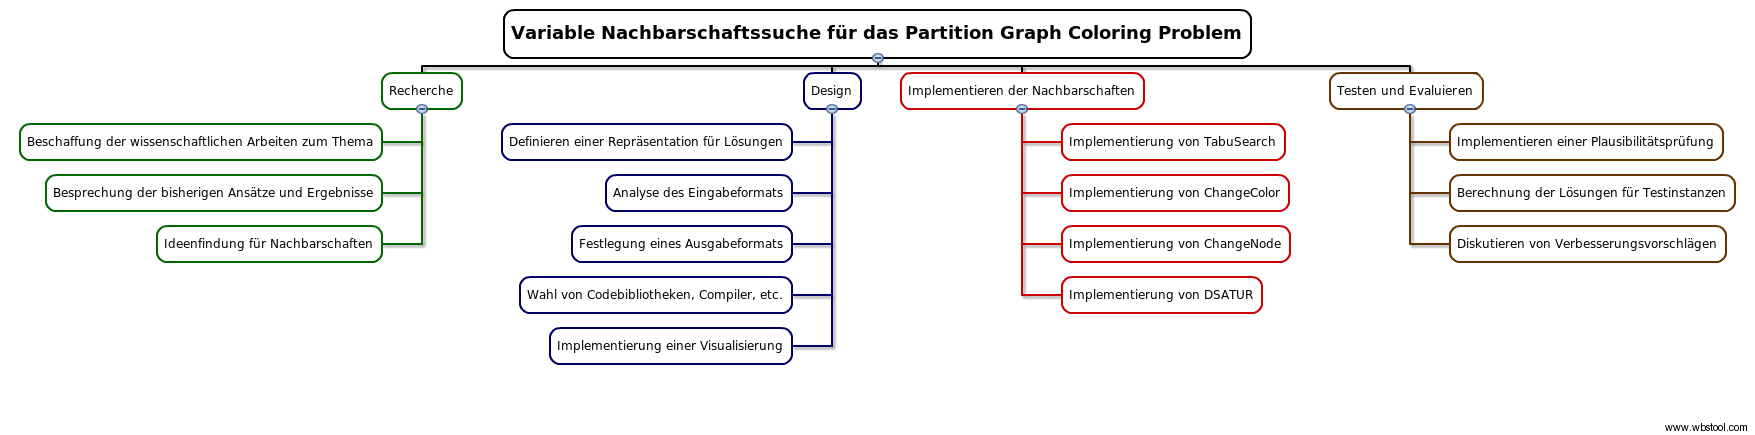
\includegraphics[angle=90, height=0.9\textheight]{img/psp.png}
\caption[Projektstrukturplan]{Projektstrukturplan zur Übersicht über die Teilaufgaben innerhalb des Projektablaufs.}
\label{fig:psp}
\end{figure}

\subsection{Recherche}

Um nicht bereits zu Projektbeginn die Fehler anderer erneut zu begehen, erschien eine ausgedehnte Recherchephase sinnvoll. Rückblickend zeigte sich diese Phase als besonders hilfreich, um mit der komplexen Materie vertraut zu werden.

\paragraph{Beschaffung der wissenschaftlichen Arbeiten zum Tehema}{Die wissenschaftliche Komponente des Projekts erforderte die umfangreiche Auseinandersetzung mit bereits abgeschlossenen Arbeiten zu ähnlichen Lösungsansätzen der gleichen Problemstellung. Am wichtigsten hierbei ist das Identifizieren von wichtigen Erkenntnisse, die sich vorteilhaft für die eigene Arbeit nutzen lassen. So konnten wir beispielsweise schnell die Konstruktionsheuristik onestepCD anderen Varianten vorziehen, da diese in früheren Evaluierungen die besten Ergebnisse berechnete.} %TODO referenz auf onestep

\paragraph{Besprechung der bisherigen Ansätze und Ergebnisse}{Abgesehen von der Wahl von onestepCD aufgrund der offensichtlichen Vorteile, wurde vorallem die Tabu-Suche von genauer analysiert, um daraus eventuell Schlüsse für leistungsfähige Nachbarschaften ziehen zu können. In der Tat führte dies zur Implementierung der Tabu-Suche als Nachbarschaft zu Testzwecken.} %TODO referenz auf onestep, referenz auf tabusearch paper

\paragraph{Ideenfindung für Nachbarschaften}{Zum Abschluss der Recherchephase entwickelte sich bereits ein Gespür für die Struktur des Problems, sodass Ideen für eigene Nachbarschaften aufkamen.} %TODO

\subsection{Design}

Nach einer Umfangreichen Recherche und Auseinandersetzung mit der Problemstellung ging das Projekt in die Designphase über. Hier galt es sicherzustellen wie die Implementierung der Nachbarschaften erfolgen soll und außerdem Schnittstellen des Programms zur Außenwelt klar zu definieren.

\paragraph{Definieren einer Repräsentation für Lösungen}{}
\paragraph{Analyse des Eingabeformats}{Eine wichtige Eingabeschnittstelle des Programms ist das Einlesen von Probleminstanzen über die Standardeingabe. Hier wurde das Parsing zweier verschiedener Quellformate implementiert. Einerseits das \texttt{.pcp}-Format, in welchem ein Großteil der Instanzen vorlagen, andererseits, das \texttt{.col}-Format.}
\paragraph{Festlegung des Ausgabeformats}{Um die Ergebnisse der Berechnungen leicht auswerten zu können, wurde die Ausgabe aller Daten im JSON-Format beschlossen. }
\paragraph{Wahl von Codebibliotheken, Compiler, etc.}{Bevor die Entwicklung des Programms tatsächlich beginnen konnte, wurde eine Codebibliothek gewählt, welche zusätzlich Zeit sparen und Fehlerquellen eindämmen würde. Weitere Details siehe \ref{sec:boost}}
\paragraph{Implementierung einer Visualisierung}{Um die Arbeitsweise des Programms möglichst anschaulich darstellen zu können, wurde eine Visualisierung mit Ubigraph implementiert. Dies ermöglicht eine Überwachung der Abreitsschritte einzelner Nachbarschaften, sodass auch Dritte Einsicht in den Ablauf gewinnen.}

\subsection{Implementierung von Nachbarschaften}

\paragraph{Implementierung von TabuSearch}{Als erstes wurde die Tabu-Suche implementiert, da eine ausführliche Beschreibung des Verfahrens vor lag.} %TODO referenz tabusuche
\paragraph{Implementierung von ChangeColor}{} %TODO moritz?
\paragraph{Implementierung von ChangeNode}{} %TODO moritz?
\paragraph{Implementierung von DSATUR}{}

\subsection{Testen und Evaluierung}

\paragraph{Implementieren einer Plausibilitätsprüfung}{Um sicher zu gehen, dass die von den Heuristiken berechneten Lösungen plausibel sind, also keine Konflikte oder unerwünschte Verbindungen enthalten, müssen diese überprüft werden. Da dies mit steigender Instanzgröße nicht von Hand möglich ist, wurde ein simpler Plausibilitätscheck implementiert.}
\paragraph{Berechnung der Lösungen für Testinstanzen}{Um die Ergebnisse des in dieser Arbeit beschriebenen Ansatzes vergleichen zu können, wurden Testinstanzen herangezogen, welche als Richtwert dienen können.}
\paragraph{Diskutieren von Verbesserungsvorschlägen}{Nach Abschluss des Projekts ist davon auszugehen, dass eine weitere Verbesserung der Ergebnisse möglich ist. In einer abschließenden Diskussion ging es darum, wie dieser Weg weiter verfolgt werden könnte.}

\section{Arbeitspakete}
\label{sec:arbeitspakete}

\begin{tabular}{cccc}
	Name & Teilnehmer & Verantwortlich & Aufwand \\
	\hline\hline\hline
	Recherche & & & \\
	\hline\hline
\end{tabular}

\section{Risikoanalyse}
\begin{table}
\centering
\begin{tabular}{lccc}
Risiko & Eintreten $p$ & Ausmaß $s$ & Priorität $P$\\
\hline
Untergang der Welt mit Ende des 13.\ Baktun & $0.5$ & $1$ & $0.5$\\
Fehlende Vergleichsmöglichkeit der Ergebnisse & $0.25$ & $0.75$ & $0.1875$ \\
Fehlende Kenntnisse in C++ & $0.2$ & $0.8$ & $0.16$ \\
Datenverlust & $0.1$ & $0.9$ & $0.09$ \\
\end{tabular}
\caption{Übersicht über identifizierte Risiken}
\label{tab:risk}
\end{table}

Wie in Tabelle \ref{tab:risk} ersichtlich ging von dem befürchteten Weltuntergang mit dem Beginn des nächsten \textit{Baktun}-Zyklus im Kalendarsystem der Maya-Hochkultur eine große Gefahr für die Erfüllung der Projektziele aus, doch die präventive Verbarrikadierung des Projektteams am 21.12.2012 konnte  durchgehende Arbeit (zu diesem Zeitpunkt an der Implementierung) gewährleisten und erwies sich im Nachhinein als nicht zwingend nötig, da beim Verlassen des Hochsicherheitssystems am 22.12.\ keine dem Ereignis zuordenbaren größeren Infrastrukturschäden im Großraum Wien bemerkt wurden.

Das Absichern gegen weitere Risikoszenarien konnte aufgrund der weit höheren Priorität im Laufe der Vorbereitungen auf den Untergang der Welt nicht gewährleistet werden.

\section{Versionskontrolle}
Eine der ersten Entscheidungen im Laufe der Arbeit am Projekt, wahrscheinlich sogar schon vor der Wahl des Arbeitstitels, war die Auswahl eines geeigneten Versionskontrollsystems. Wie es die Teammmitglieder für kleinere Projekte gewohnt war, begann die Entwicklung in einem von einem Cloud Service bereitgestellten, synchronisierten Ordner. Doch schon nach wenigen Tagen war klar, dass eine für das Projektteam derart wichtige Arbeit ein voll ausgebautes und dezidiertes Versionskontrollsystem benötigt. Schnell fiel die Entscheidung auf \textit{Git}\footnote{\url{https://git-scm.org/}}, ein System, dass mitunter von den Entwicklern der größten Projekte der \textit{Free and/or Open Source Software} eingesetzt wird.

Dabei beeindruckt Git vorallem durch den geringen Mehraufwand um die Versionskontrolle zu pflegen. Weiters wurde es so möglich komplett unabhängig an Dateien zu arbeiten und Änderungen im Nachhinein einfach zusammenzuführen.

\section{Continuous Integration}
Als zusätzliches Feedback-Element wurde in diesem Projekt auf Continuous Integration gesetzt. Das bedeutet, dass sobald Änderungen am Code in der Versionskontrolle eingecheckt und hochgeladen wurden, ein Webservice zur Verfügung stand um die neue Version zu kompilieren und zu testen. Bei fehlschlagen eines solchen Builds wurde das Projektteam instantan informiert um möglichst rasch eine Fehlerbehebung zu beginnen.

Dies ermöglicht insbesondere auch die Überprüfung, ob der Code sich mit GCC genauso wie mit clang kompilieren lässt und bietet außerdem einen guten Richtwert der im Projektlauf aufgetretenen Fehler. 

\newpage
\addcontentsline{toc}{chapter}{Verzeichnisse}
\printbibliography[title=Literaturverzeichnis]
\addcontentsline{toc}{section}{Literaturverzeichnis}
\listoffigures
\addcontentsline{toc}{section}{Abbildungsverzeichnis}
\listoftables
\addcontentsline{toc}{section}{Tabellenverzeichnis}
\listofalgorithms
\addcontentsline{toc}{section}{Algorithmenverzeichnis}
\lstlistoflistings
\addcontentsline{toc}{section}{Codeverzeichnis}
\appendix

\chapter{Ergebnisse}

Eine Auswahl der bisherigen Ergebnisse unseres Projektes auf aus der wissenschaftlichen Li\-te\-ra\-tur für dieses Optimierungsproblem bekannten Instanzen können der Tabelle~\ref{tab:result} entnommen werden, die Bedeutung der einzelnen Spalten ist wie folgt:

\begin{description}
    \item[Instanz] Name der berechneten Instanz\footnote{Zu finden unter \url{www.ic.uff.br/~celso/grupo/pcp.htm}}.% In dem Format \texttt{n}\textit{(Anzahl der Knoten)}\texttt{}
    \item[$|V|$] Anzahl der Knoten der Instanz.
    \item[$|E|$] Anzahl der Kanten der Instanz.
    \item[$|C|$] Anzahl der Clustern der Instanz.
    \item[$S_i$] Die Anzahl der Farben, die von der durch \emph{onestepCD} berechneten Ausgangslösung benötigt werden.
    \item[$N$] Die verwendeten Nachbarschaften in Reihenfolge der Iteration:
        \begin{description}
            \item[\texttt{c}] \emph{ChangeColor}
            \item[\texttt{n}] \emph{ChangeNode}
            \item[\texttt{d}] \emph{DSATUR}
        \end{description}
    \item[$S_{avg}$] Die im Durchschnitt benötigte Anzahl an Farben der von unserer Implementierung in 30 Testläufen berechneten Lösungen.
    \item[$S_{\sigma}$] Die Standardabweichung der Ergebnisse aller Testläufe (verursacht durch Ran\-dom\-isier\-ung in den einzelnen Verfahren).
    \item[$S_{\Delta}$] Prozentuelle Verbesserung der Ausgangslösung durch den beschriebenen Ansatz.
    \item[$t$] Mittlere Laufzeit in Sekunden (ermittelt auf einem Linux-System Kernel 3.5.0 x86\_64, Intel Core i5-3317U CPU mit 1.70GHz, Compiler gcc 4.7.2 ).
\end{description}

\paragraph{Kurzinterpretation}{Wie man erkennen kann ist die Reihenfolge, in der das VND die einzelnen Nachbarschaften durchsuchen muss, um die jeweils besten Resultate zu erzielen, nicht wirklich eindeutig, auch wenn sich eine Tendenz zu \texttt{cnd} abzeichnet. Die erzielten Verbesserung gegenüber der von der Konstruktionsheuristik \emph{onestepCD} ermittelten Ausgangslösungen sind mitunter beachtlich und bewegen sich großteils im Bereich zwischen 20 und 40\%.}

\begin{table}[!htbp]
\centering
\begin{tabular}{c|rrr|r|c|rrr|r|r}
Instanz & $|V|$ & $|E|$ & $|C|$ & $S_i$ & $N$ & $S_{min}$ & $S_{avg}$ & $S_{\sigma}$ & $S_{\Delta}$ & $t$ \\
\hline\hline
\texttt{n90p5t2s1.pcp} & 90	& 2019	& 45 & 13 & \texttt{cdn} & 9 & 9.61 & 1.8 & 44.44 & 693.2\\
\texttt{n90p5t2s2.pcp} & 90	& 1963	& 45 & 11 & \texttt{ncd} & 8 & 9.29 & 1.8 & 37.50 & 550.6\\
\texttt{n90p5t2s3.pcp} & 90	& 2045	& 45 & 13 & \texttt{cdn} & 9 & 9.61 & 1.8 & 44.44 & 568.4\\
\texttt{n90p5t2s4.pcp} & 90	& 2014	& 45 & 12 & \texttt{cdn} & 9 & 9.61 & 1.8 & 33.33 & 593.9\\
\texttt{n90p5t2s5.pcp} & 90	& 2057	& 45 & 13 & \texttt{dnc} & 9 & 9.87 & 1.9 & 44.44 & 789.7\\
\texttt{n90p7t2s4.pcp} & 90	& 2821	& 45 & 16 & \texttt{ndc} & 12 & 13.35 & 2.5 & 33.33 & 656.1\\
\texttt{n90p7t2s5.pcp} & 90	& 2834	& 45 & 16 & \texttt{cdn} & 13 & 13.94 & 2.6 & 23.08 & 847.7\\
\texttt{n90p8t2s1.pcp} & 90	& 3257	& 45 & 19 & \texttt{dcn} & 15 & 16.77 & 3.2 & 26.67 & 839.0\\
\texttt{n90p8t2s2.pcp} & 90	& 3188	& 45 & 19 & \texttt{cdn} & 15 & 16.06 & 3.0 & 26.67 & 1125.5\\
\texttt{n90p9t2s1.pcp} & 90	& 3631	& 45	& 24 & \texttt{cnd} & 19 & 20.48 & 3.8 & 26.32 & 1247.4\\
\texttt{n90p9t2s2.pcp} & 90	& 3614	& 45	& 23 & \texttt{cnd} & 18 & 20.42 & 3.9 & 27.78 & 1051.3\\
\texttt{n90p9t2s3.pcp} & 90	& 3615	& 45	& 24 & \texttt{cdn} & 19 & 19.97 & 3.7 & 26.32 & 1432.6\\
\texttt{n90p9t2s4.pcp} & 90	& 3619	& 45	& 23 & \texttt{dcn} & 17 & 19.77 & 3.8 & 35.29 & 1407.4\\
\texttt{n90p9t2s5.pcp} & 90	& 3634	& 45	& 24 & \texttt{dcn} & 18 & 19.42 & 3.6 & 33.33 & 1357.1\\
\texttt{n100p5t2s1.pcp} & 100	& 2494	& 50	& 13 & \texttt{cdn} & 10 & 10.58 & 2.0 & 30.00 & 689.7\\
\texttt{n100p5t2s2.pcp} & 100	& 2428	& 50	& 12 & \texttt{cdn} & 10 & 10.55 & 1.9 & 20.00 & 489.0\\
\texttt{n100p5t2s3.pcp} & 100	& 2513	& 50	& 12 & \texttt{ndc} & 9 & 9.94 & 1.9 & 33.33 & 610.6\\
\texttt{n100p5t2s4.pcp} & 100	& 2442	& 50	& 12 & \texttt{cdn} & 9 & 9.94 & 1.9 & 33.33 & 602.3\\
\texttt{n100p5t2s5.pcp} & 100	& 2500	& 50	& 12 & \texttt{dnc} & 9 & 10.55 & 2.1 & 33.33 & 848.7\\
\texttt{n120p5t2s1.pcp} & 120	& 3593	& 60	& 14 & \texttt{cdn} & 11 & 12.03 & 2.3 & 27.27 & 1549.0\\
\texttt{n120p5t2s2.pcp} & 120	& 3544	& 60	& 14 & \texttt{cdn} & 11 & 11.77 & 2.2 & 27.27 & 906.8\\
\texttt{n120p5t2s3.pcp} & 120	& 3613	& 60	& 14 & \texttt{cdn} & 12 & 11.90 & 2.2 & 16.67 & 651.0\\
\texttt{n120p5t2s4.pcp} & 120	& 3536	& 60	& 14 & \texttt{dcn} & 11 & 11.87 & 2.2 & 27.27 & 1334.2\\
\texttt{n120p5t2s5.pcp} & 120	& 3623	& 60	& 15 & \texttt{ndc} & 11 & 12.23 & 2.3 & 36.36 & 1050.3\\
\end{tabular}
\caption{Ergebnisse der VNS im Überblick}
\label{tab:result}
\end{table}

\end{document}
